\chapter{Data acquisition}

In nuclear medicine, photon detection hardware differs considerably from that
used in CT. In CT, large numbers of photons must be acquired in a very short
measurement. In emission tomography, a very small number of photons is
acquired over a long time period. Consequently, emission tomography systems are
optimized for sensitivity.

Photo-electric absorption is the preferred interaction in the detector, since
it results in absorption of all the energy of the incoming photon. Therefore
the detector material must have a high atomic number (the atomic number Z is
the number of electrons in the atom). Since interaction probability decreases
with increasing energy, a higher Z is needed for higher energies.

In single photon imaging, \textsuperscript{99m}Tc\ is the tracer that is mostly used. It has
an energy of 140 keV and the gamma camera performance is often optimized for
this energy.  Obviously, PET-cameras have to be optimized for 511~keV.

\section{Detecting the photon}
%%%%%%%%%%%%%%%%%%%%%%%%%%%%%%
Different detector types exist, but the current standard, both in SPECT and
PET, is the scintillation detector. The following sections describe the
scintillation crystal, the photomultiplier tube and how crystal and tubes
can be combined to make a two-dimensional gamma detector. After that, some
alternative designs and new developments will be mentioned.

\subsection{Scintillation crystal}
%=================================
A scintillation crystal is a remarkable material that stops the incoming
photon and in doing so produces a flash of visible light, a scintillation.
So the problem of detecting the incoming photon is now transformed in the
easier problem of detecting the light flash.

The scintillation stops the photon via photo-electric absorption or via
multiple scattering events. The resulting photo-electron travels through the
crystal, distributing its kinetic energy over a few thousands other electrons
in multiple collisions. As a result, there will be a few thousands of a
electrons in an excited state. After a short time, these electrons will
release their energy in the form of a photon of a few eV. These secondary
photons are visible to the human eye (they are usually blue): this is the
scintillation.

The exact wavelength (or color) of the light flash depends on the crystal,
but {\em not} on the energy of the incoming high-energy photon. If a photon
with a higher energy enters the crystal, it will send more electrons to an
higher energy level. Each of these electrons will then produce a single
scintillation-photon, always with the same color. So if we want to have an
idea about the energy of the incoming photon, we need to look at the number
of scintillation photons (the intensity of the flash), and not at their
energy (the color of the flash).

Many scintillators exist, and quite some research on new scintillators
is still going on. The crystals that are mostly used today are NaI(Tl)
for single photons (140 keV) in gamma camera and SPECT, and LSO
(lutetium oxyorthosilicate) for annihilation photon (511 keV) in
PET. Before LSO was found, BGO (bismuth germanate) was used for PET,
and there are still some old BGO-based PET systems around. Some other
crystals, such as GSO (gadolinium oxyorthosilicate) and LYSO (LSO with
a bit of Yttrium, very similar to LSO) are used for PET as well. The
important characteristics of the crystals are:
\begin{itemize}
  \item Transparency. If it is not transparent, we cannot see or detect the
        light flash.
  \item Photon yield per incoming keV. More photons per keV is better, since
        the light flash will be easier to see. The scintillation and
        its detection are statistical processes, and the uncertainty
        associated with it will go down if the number of scintillation
        photons increases.
  \item Scintillation time. This is the average time that the electrons
        remain in the excited state before releasing the scintillation
        photon. Shorter is better, since we want to be ready for the next
        photon.
  \item Attenuation coefficient for the high energy photon. We want to stop
        the photon, so a higher attenuation coefficient is better. Denser
        materials tend to stop better.
  \item Wave length of the scintillation light. Some wave lengths are easier
        to detect than others.
  \item Ease of use: some crystals are very hygroscopic: a bit of water
        destroys them. Others can only be produced at extremely high
        temperatures. And so on.
\end{itemize}

\begin{table}
\centering
\caption{Characteristics of a few scintillation crystals.}
\label{tab:crystals}
\begin{tabular}{|c|c|c|c|c|}
\hline
       & NaI(Tl) &    BGO      & LSO      & GSO \\
\hline
Photons per keV                    
        &  40     & 5 \ldots 8  & 20 \ldots 30 &  12\\
Scintillation decay time [ns]
        & 230     &  300  & 40  & 65 \\
Linear atten. coeff. [/cm] (at 511 keV)
        & 0.34    & 0.95  & 0.87  & 0.67\\
 Wave length [nm]
        & 410     & 480   & 420 & 440 \\
Melting temperature ($^o$C)
        & 651 & 1050 & 2050 & 1950 \\
\hline
\end{tabular}
\begin{itemize}
\item NaI(Tl): NaI crystal doped with Tl
\item BGO: Bi$_4$Ge$_{3}$O$_{12}$
\item LSO: Lu$_2$SiO$_5$
\item GSO: Gd$_2$SiO$_5$ doped with Ce
\end{itemize}
\end{table}

The scintillation photons are emitted to carry away the energy set
free when an electron returns to a lower energy level. Consequently,
these photons contain just the right amount of energy to drive an
electron from a lower level to the higher one. In pure NaI this
happens all the time, so the photons are reabsorbed and the
scintillation light never leaves the crystal. To avoid this, the NaI
crystal is doped with a bit of Tl (Thallium). This disturbs the
lattice and creates additional energy levels. Electrons returning to
the ground state via these levels emit photons that are not
reabsorbed.  NaI is hygroscopic (similar as NaCl (salt)), so it must
be protected against water. LSO has excellent characteristic, but is
difficult to process (formed at very high temperature), and it is
slightly radioactive. Table \ref{tab:crystals} lists some
characteristics of three scintillation crystals.

\subsection{Photo Multiplier Tube}
%=================================
The scintillation crystal transforms the incoming photon into a light flash.
That flash must be detected. In particular, we want to know {\em where} it
occurred, {\em when} it occurred and {\em how intense} it was (to compute the
energy of the incoming photon). All this is usually obtained with
photomultiplier tubes (PMT).

\begin{figure}[tb]
\centering
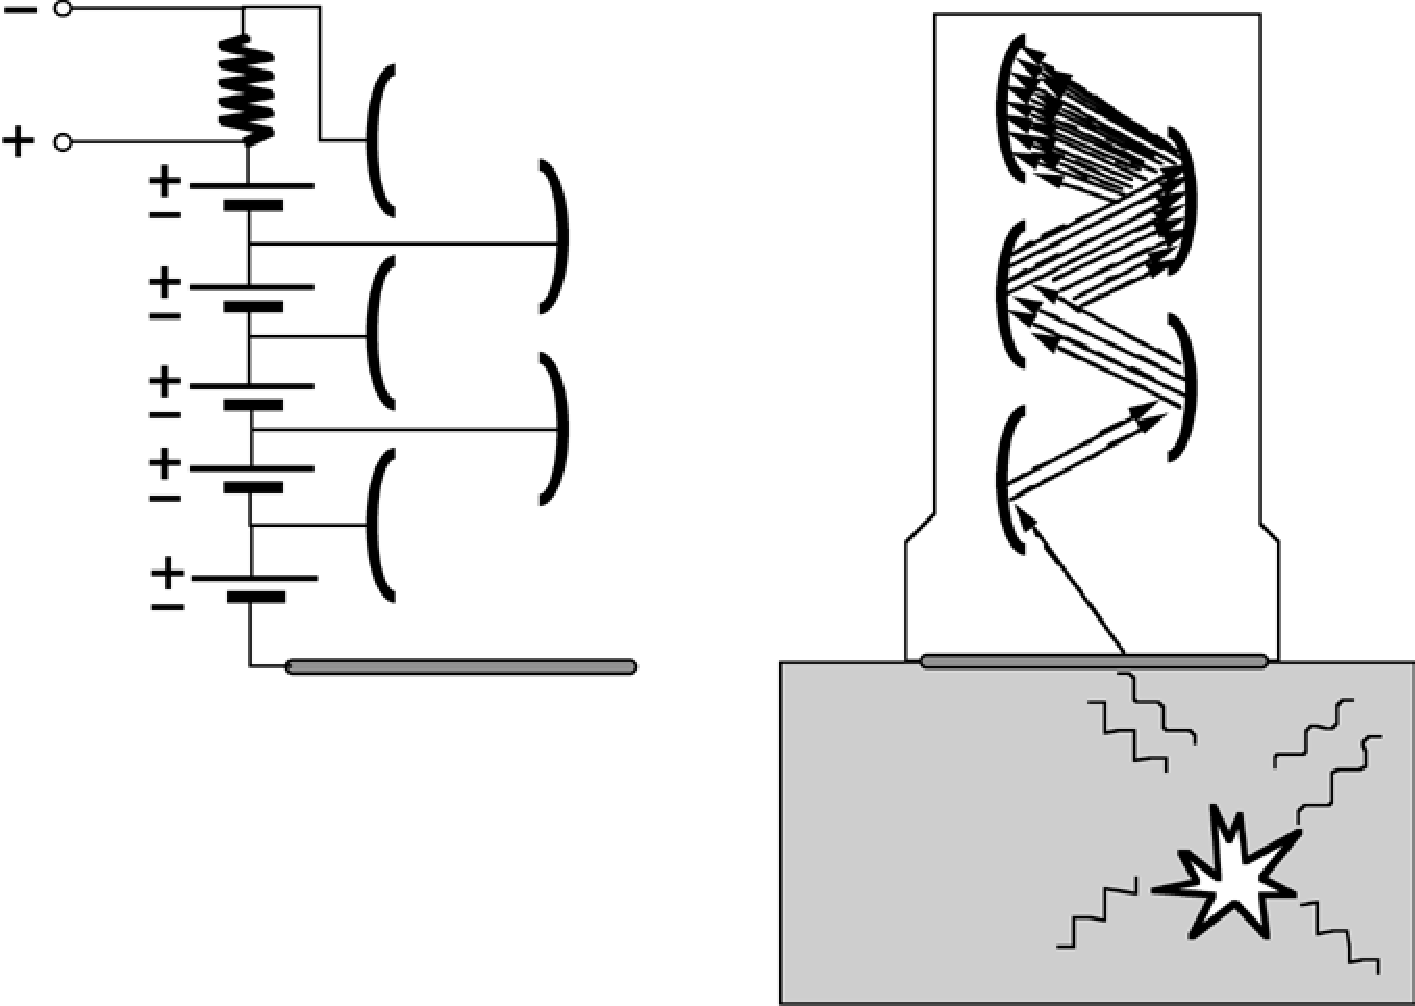
\includegraphics[width=0.5\textwidth]{figs/fig_jnpmt.pdf}
\caption{\label{fig:jnpmt} \emph{Photomultiplier. Left: the electrical scheme.
Right: scintillation photons from the crystal initiate an electric current to
the dynode, which is amplified in subsequent stages.}}
\end{figure}

The PMT's are glued onto the crystal, in order to detect the incoming
scintillation photons. The PMT consists of multiple dynodes, the first of
which (the photocathode) is in optical contact with the crystal. High negative
voltage (in the order of 100 V) between the dynodes makes the electrons want
to jump from one to the other, but they do not have enough energy to cross the
gap in between (fig \ref{fig:jnpmt}).  This energy is provided by the
scintillation photon. The electron acquiring the threshold energy will be
accelerated by the electrical field, and activate multiple electrons in the
next dynode. After a few steps, a measurable voltage is created which is
digitized with an analog-to-digital converter. There are usually about 10 to
12 dynodes, and each step amplifies the signal with a factor 3 \ldots 6, so
amplification can be in the order of one million.

The response time of a PMT is very short (a few ns) compared to the
scintillation decay time.


\subsection{Two-dimensional gamma detector}
%==========================================
% Single crystal vs multicrystal
% position (intrinsic resolution), energy (-resolution)
% constant fraction discriminator.
%
There are two ways to build a two-dimensional gamma detector based on
scintillation. One way is to use a single very large crystal and connect
multiple PMT's to it. The other way is to combine small crystals in a
large matrix.

\subsubsection{Single crystal detector} \label{sec:single_crystal}
%------------------------------------
This is the standard design for single photon detectors with NaI(Tl). One
side of a single large crystal (e.g. 50 cm x 40 cm, 1 cm thick) is covered
completely with PMT's (\ldots 50 \ldots PMTs). The other side is covered with
a layer acting as a mirror for the scintillation photons, so that as many as
possible are collected in the PMT's.

In principle, all PMT's contribute to the detection of a single
scintillation event. As mentioned before, the position, the time and the
energy ( $\sim$ amount of scintillation photons) must be computed from the
PMT-outputs.
%
\begin{itemize}

\item {\bf Position:} $(x,y)$\\
The x-position is computed as
\begin{equation}
x = \frac{\sum_i x_i S_i}{\sum_i S_i}, \label{eq:gammaposition}
\end{equation}
where $i$ is the PMT-index, $x_i$ the $x$-position of the PMT and $S_i$ the
integral of the PMT output over the scintillation duration.  The $y$-position
is computed similarly. Expression (\ref{eq:gammaposition}) is not very
accurate and needs correction for systematic errors (linearity correction).
The reason is that the response of the PMT's does not vary nicely with the
distance to the pulse. In addition, each PMT behaves a bit differently. This
will be discussed later in this chapter.

\item {\bf Energy:} $E$\\
The energy is computed as
\begin{equation}
 E = c_E {\sum_i S_i}
\end{equation}
where $c_E$ is a coefficient converting voltage (integrated PMT output) to
energy. The ``constant'' $c_E$ is not really a constant: it varies slightly
with the energy of the high energy photon. Moreover, it depends also on
the position of the scintillation, because of the complex and individual
behavior of the PMT's. Compensation of all these effects is called ``energy
correction'', and will be discussed below.

\item {\bf Time: } $t$\\
In positron emission tomography, we must detect pairs of photons which have
been produced simultaneously during positron-electron annihilation.
Consequently, the time of the scintillation must be computed as accurately as
possible, so that we can separate truly simultaneous events from events that
happen to occur almost simultaneously.

The scintillation has a finite duration, depending on the scintillator
(see table \ref{tab:crystals}).  The scintillation duration is
characterized by the the decay time $\tau$, assuming that the number
of scintillation photons decreases as $\exp(- t/\tau)$. The decay
times of the different scintillation crystals are in the range of 40
to several 100 ns. This seems short, but since a photon travels about
1 meter in only 3.3 ns, we want the time resolution to be in the order
of a few ns (e.g. to suppress the random coincidence rate in PET, as
will be explained in section \ref{sec:septa}). To assign such a
precise time to a relatively slow event, the electronics typically
computes the time at which a predefined fraction of the scintillation
light has been collected (constant fraction discriminator). In current
time-of-flight PET systems based on LSO, one obtains a timing
resolution of about 400 ps.

\end{itemize}

\subsubsection{Multi-crystal detector matrix}
%------------------------------------
Instead of using a single large crystal, a large detector area can be
obtained by combining many small crystals in a two-dimensional
matrix. The crystals should be optically separated (such that
scintillation photons are mirrored at the edges), to make sure that
the scintillation light produced in one crystal stays in that
crystal. In the extreme case, each crystal has its own
photomultiplier. Computation of position is ``trivial'' (although
complicated in practice): it is the coordinate of the crystal in the
matrix (no attempt is made to obtain sub-crystal accuracy). Energy is
proportional to the total output of the PMT coupled to the crystal. In
such a design, the top of the crystal is usually a square of 3 to 5
mm, and the crystal is a cm (140 keV) or a few cm (511 keV) thick.
Consequently, the spatial resolution is about 4 mm, as in the single
crystal case (see section \ref{sec:resolution}).

\begin{figure}[tb]
\centering
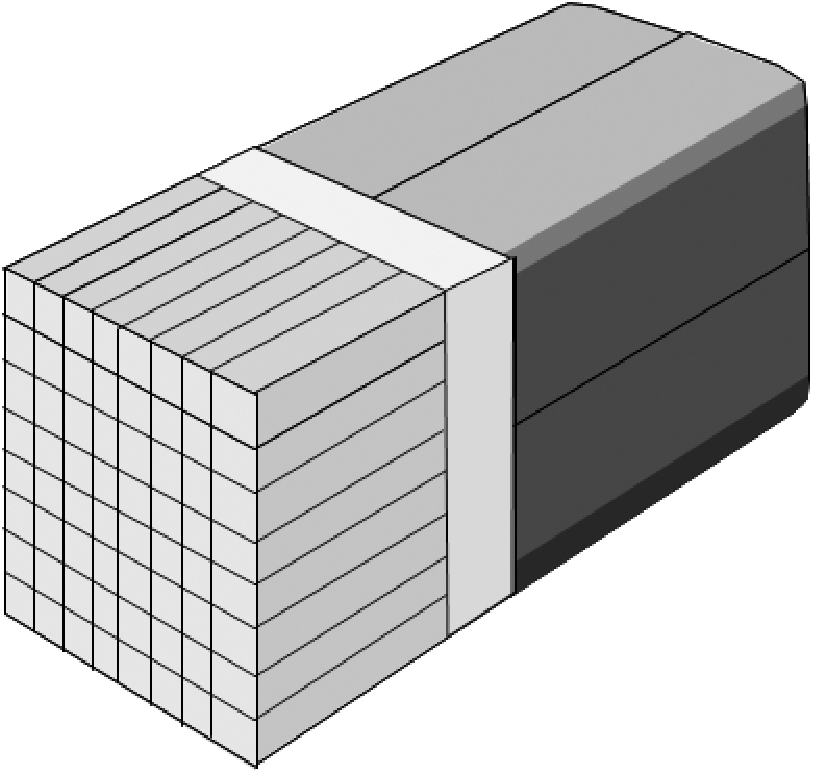
\includegraphics[width=0.3\textwidth]{figs/fig_multicrystal.pdf}
\caption{\label{fig:multicrystal} \emph{Multi-crystal module. The outputs
of four photomultipliers are used to compute in which of the 64 crystals
the scintillation occurred.}}
\end{figure}

Photomultipliers are expensive, so the manufacturing cost can be
reduced by a more efficient use of the PMT's. Figure
\ref{fig:multicrystal} shows a typical design, where a matrix of 64
(or more) crystals is connected to only four multipliers. The
transparent block between the crystals and the PMT is called the {\em
light guide}.  It guides the light towards the PMT's in such a way
that the PMT amplitude changes monotonically with distance to the
scintillating crystal. Thus, the relative amplitudes of the four
PMT-outputs allow to compute in which crystal the scintillation
occurred. For PET, the crystals have typically a cross section of
about 4mm $\times$ 4 mm, and they are about 2 cm long.

In a single crystal design, all PMT's contribute to the detection of a single
scintillation. If two photons happen to hit the crystal simultaneously, both
2scintillations will be combined in the calculations and the resulting energy
and position will be wrong! Thus, the maximum count rate is limited by the
decay time of the scintillation event. In a multi-crystal design, many modules
can work in parallel, so count rates can be much higher than in the single
crystal design. Count rates tend to be much higher in PET than in SPECT or
planar single photon imaging (see below). That is why most PET-cameras are
using the multicrystal design, and gamma cameras are mostly single crystal
detectors. However, single crystal PET systems and multi-crystal gamma cameras
exist as well.


\subsection{Resolution} \label{sec:resolution}
%=================================
The coordinates $(x, y, E, t)$ can only be measured with limited precision.
They depend on the actual depth where the incoming photon was stopped, on
the number of electrons that was excited, on the time the electrons remain
in the excited state, on the direction in which each scintillation photon is
emitted when the electron returns to a lower energy state and on the amount of
electrons that is activated in the PMT's in each dynode. These are all
random processes: if two identical high energy photons enter the crystal at
exactly the same position, all the forthcoming events will be different. We
can only describe them with probabilities.

So if the photon really enters the crystal at $(\bar{x}, \bar{y}, \bar{E},
\bar{t})$, the actual measurement will produce a random realization $(x_i,
y_i, E_i, t_i)$ drawn from a four-dimensional probability distribution
$(x, y, E, t)$. We can measure that probability distribution by doing
repeated measurements in a well-controlled experimental situation. E.g., we
can put a strongly collimated radioactive source in front of the crystal,
which sends photons with the same known energy into the crystal at the same
known position. This experiment would provide us the distribution for $x$,
$y$ and $E$. The time resolution can be determined in several ways, e.g. by
activating the PMT's with light emitting diodes. The resolution on $x$ and $y$
is often called the {\em intrinsic resolution}.

If we plot all the measurements in a histogram, we will see the
distribution. Usually the distribution is approximately Gaussian, and can be
characterized by its standard deviation $\sigma$. Often one specifies the
full width at half maximum (FWHM) instead (figure \ref{fig:fwhm}). It is easy
to show that for a Gaussian, the FWHM $ = 2 \sqrt{2 \ln 2} \sigma$. This
leads to a useful rule of thumb: {\em any detail smaller than the FWHM is lost
during the measurement}.
 
\begin{figure}[tb]
\centering
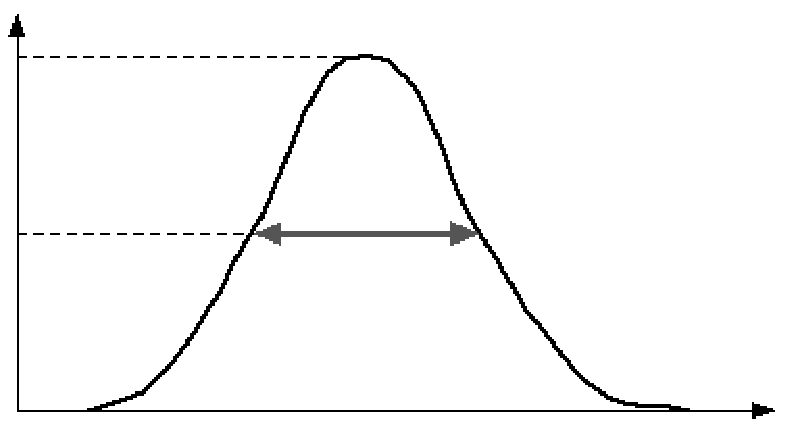
\includegraphics[width=0.35\textwidth]{figs/fig_fwhm.pdf}
\caption{\label{fig:fwhm} \emph{The full width at half max of a probability
distribution}}
\end{figure}

Position resolution of a scintillation detector has a FWHM of 3 to 4 mm.
Energy resolution is about 10\% FWHM (so 14 keV for a 140 keV tracer) in
NaI(Tl) cameras, about 20\% FWHM (about 130 keV at 511 keV) or worse in
BGO PET-systems, and about 15\% FWHM in LSO and GSO PET-systems.

\subsection{Storing the data} \label{sec:storing_data}
%=================================
To store the data, the information must be digitized. We do not want to lose
information, so the round-off errors made during digitization should be small
compared to the resolution. Thus, we obtain four digital numbers $(x, y, E,
t)$, which are the coordinates of a single detected photon. If all information
must be preserved, we can directly store the four numbers in a list (list-mode
acquisition). Obviously, this list may become very long. Often, we do not need
all this information. The energy is usually simply used to decide whether we
will accept or discard the photon, it does not need to be stored (this will be
explained in section \ref{sec:scatter}). Similarly, we often want to
make a single image representing the situation in a certain time interval, so
we only need a single two-dimensional image. To store this information
efficiently, we prepare a zero two-dimensional matrix, an ``empty'' image, and
increment the value at coordinates $x_i, y_i$ for the $i$-th accepted
photon. The number can be interpreted as a brightness, so we can display the
result as an image on the screen. Brightness (or some pseudo-color)
corresponds to tracer concentration.


\subsection{Alternative designs}
%=================================
Although most current gamma cameras and PET systems are based on
scintillation crystals combined with photomultipliers, there are many
other detection systems. Some of these have very good characteristics, but
their acceptance is hampered by the high cost price and, in some cases, by
the fact that new algorithms must be developed before their full potential
can be exploited. In the following, we only mention two promising
technologies. Avalanche photodiodes can replace the PMT, CdZnTe detectors
can replace the entire standard detection system.

\subsubsection{Avalanche photodiodes}
%------------------------------------
A semiconductor is a material in which the large majority of electrons are
strongly bound to the atoms, but not all of them. Some electrons have enough
energy to move freely about as in a metal. As a result, some of the atoms
have lost an electron and have a net positive charge. This phenomenon gives
rise to two types of charge carriers that can support electric current:
electrons and holes. The former are the freely moving electrons. The latter
are the positive vacancies left behind by the electrons. The holes can move,
because an electron from a neighboring atom can jump over to fill in the
vacancy, creating a similar vacancy in the neighboring atom.

Electric current is possible if freely moving electrons or holes are
available. However, if for some reason none of them are available, the
material acts as an insulator.

A diode is a simple electronic device with wonderful behavior. It has
excellent conductivity in one direction, and extremely poor conductivity in
the other.  This remarkable feature is obtained by connecting two very
different types of semiconductor materials, resulting in a very asymmetrical
distribution of charge carriers. When forward voltage is applied, charge
carriers are injected in great numbers, leading to very low resistance. When
reverse voltage is applied, the electrons and holes are pulled away from the
junction, so there is nothing left to support an electric
current. Consequently, it behaves as an insulator in this mode.

In an avalanche photodiode (APD), a very high reverse voltage is applied,
pulling away all charge carriers. However, a photon hitting the diode may
supply enough energy to break the covalent bond of an electron, thus
creating an electron-hole pair. This free electron will move rapidly in the
electric field, releasing other electrons from their bond. Consequently, the
photon creates an avalanche of free electrons, resulting in a measurable
current. The current is proportional to the number of electrons in the
avalanche, which in turn is proportional to the number of
scintillation photons.

APD's can be used to replace the photomultiplier. The advantage is
that they are much smaller, but currently they are still more
expensive than the PMTs. Another advantage is that they can be used in
a strong magnetic field, while PMTs cannot. In hybrid PET/MRI systems,
where the PET is operated inside the MRI-system, APDs or other similar
devices must be used instead of PMTs.

A limitation of the APD is the long response time. Their timing
resolution is not good enough for time-of-flight PET.

\subsubsection{Multi-pixel photon counters (MPPC or SiPM)}
%-------------------------------------------------
A MPPC or Silicon Photomultiplier (SiPM) consists of an array of APDs
which are operated in Geiger mode. This Geiger mode is obtained by
using a relatively high voltage, such that an incoming photon will
always create a maximum avalanche of electrons, independent of its
energy. Thus, each Geiger mode APD can count the number of
scintillation photons it is hit by. Because a single SiPM consists of
many small APDs, the likelihood of multiple photons hitting the same
APD simultaneously is small. Consequently, the SiPM reliably counts
the number of scintillation photons hitting it.

Compared to the regular APD, the SiPM has the advantage of being much
faster, achieving a response time similar to that of analogue
photomultiplier tubes. That makes them fast enough for time-of-flight
PET. Current timing resolution is around 400 ps, and prototypes with
still better timing are currently being developed.

\subsubsection{Solid state detectors}
%------------------------------------
An effect similar to the one described above can be used to directly
detect the high energy photon instead of the scintillation
photons. For this purpose, a material with high stopping power is
required. This is the operating principle of the CdZnTe detector: a
strong electric field drives charge carriers created by the high
energy photon towards a grid of collectors.  Position resolution is
now determined by the size of the collectors. Designs with
sub-millimeter resolution exist. Energy resolution is excellent (3 \%,
as opposed to the 10 \% in NaI(Tl)). The stopping power is similar to
that of NaI(Tl). Currently, the main disadvantage of CdZnTe detectors
is their very high cost.

As will be discussed in the next section, the resolution of a camera is
dominated by the collimator acceptance angle. Consequently, the excellent
spatial resolution of the CdZnTe detector is completely wasted in the
traditional design. Some researchers are studying alternative camera
designs and accompanying algorithms to fully exploit the excellent
performance of this type of detectors.


\section{Collimation}
%%%%%%%%%%%%%%%%%%%%%
% PSF. Combinatie van resoluties.
% PET sensitiever dan spect. Dus hogere count rates bij zelfde activiteit.

At this point, we know how the position and the energy of a photon
impinging on the detector can be determined. Now we need a way to
ensure that the impinging photons will produce an image. In
photography, a lens is used for that purpose. But there are no
easy-to-use lenses to focus the high energy photons used in nuclear
medicine. So we must fall back on a more primitive approach:
collimation. Collimation is the method used to make the detector
``see'' along straight lines. Different tomographic systems use
different collimation strategies, as shown in figure
\ref{fig:spect_pet_ct}.

\begin{figure}[tb]
\centering
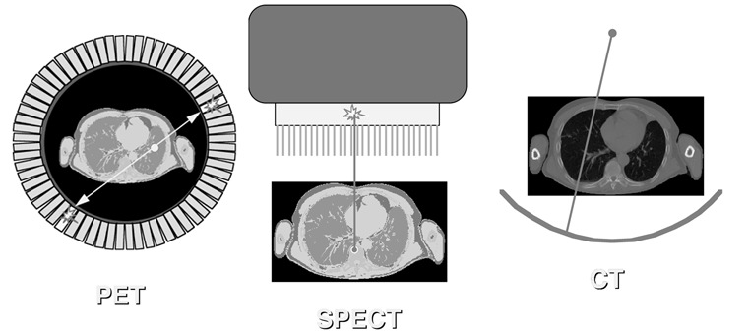
\includegraphics[width=0.75\textwidth]{figs/fig_spect_pet_ct.pdf}
\caption{\label{fig:spect_pet_ct} \emph{Collimation in the PET camera, the
gamma camera (SPECT) and the CT camera.}}
\end{figure}

In the CT-camera, collimation is straightforward: there is only one
transmission source, so any photon arriving in the detector has traveled along
the straight line connecting source and detector. In the PET-camera, a similar
collimation is obtained: if two photons are detected simultaneously, we can
assume they have originated from the same annihilation, which must have
occurred somewhere on the line connecting the two detectors. But for the gamma
camera there is a problem: only one photon is detected, and there is no simple
way to find out where it came from. To solve that problem, mechanical
collimation is used. A mechanical collimator is essentially a thick sieve with
long narrow holes separated by thin septa. The septa are made from a material
with strong attenuation (usually lead), so photons hitting a septum will be
eliminated, mostly by photo-electric interaction. Only photons traveling along
lines parallel to the collimator holes will reach the detector. So instead of
computing the trajectory of a detected photon, we eliminate all trajectories
but one, so that we know the trajectory even before the photon was detected.
Obviously, this approach reduces the sensitivity of the detector, since many
photons will end up in the septa. This is why a PET-system acquires more
photons per second than a gamma camera, for the same activity in the field of
view.

Most often, the parallel hole collimator is used, but for particular
applications other collimators are used as well. Figure \ref{fig:collimators}
shows the parallel hole collimator (all lines parallel), the fan beam
collimator (lines parallel in one plane, focused in the other), the cone beam
collimator (all lines focused in a single point) and the pin hole collimator
(single focus point, but in contrast with other collimators, the focus is
placed {\em before} the object).

\begin{figure}[tb]
\centering
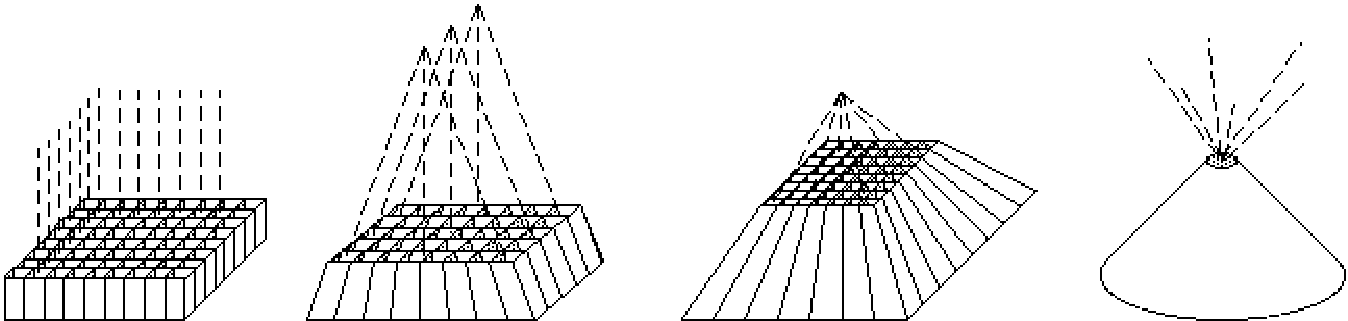
\includegraphics[width=0.6\textwidth]{figs/fig_collimators.pdf}
\caption{\label{fig:collimators} \emph{Parallel hole, fan beam, cone beam and
pin hole collimators.}}
\end{figure}

Collimation ensures that tomographic systems collect information about
lines.  In CT, detected photons provide information about the total
attenuation along the line. In gamma cameras and PET cameras, the
number of detected photons provides information about the total
radioactivity along the line (but of course, this information is
affected by the attenuation as well). Consequently, the acquired
two-dimensional image can be regarded as a set of line integrals of a
three dimensional distribution. Such images are usually called {\em
projections}.

\subsection{Mechanical collimation in the gamma camera} \label{sec:collimation}
%====================================================
Figure \ref{fig:lenscollimator} shows that the sensitivity obtained
with a mechanical collimation is very poor compared to that obtained with a
lens. The mechanical collimator has a dominating effect on the resolution and
sensitivity of the gamma camera. That is why a more detailed analysis of the
collimator point spread function is in order.

\begin{figure}[tb]
\centering
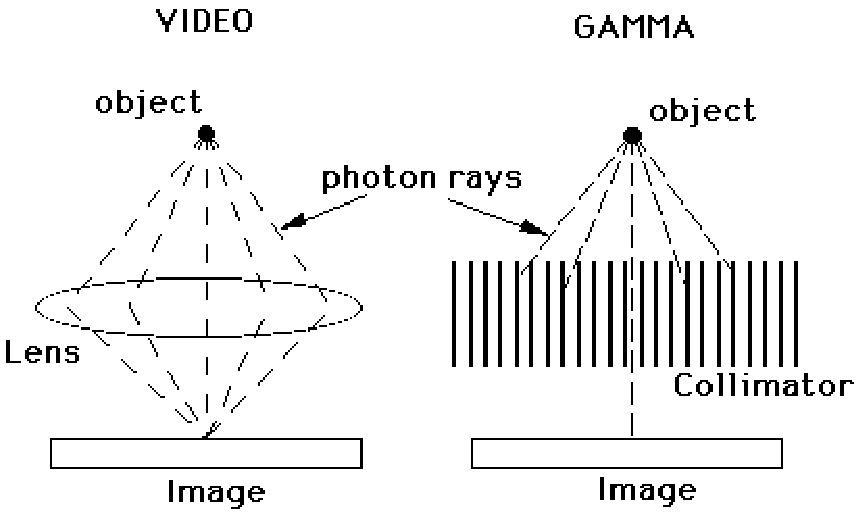
\includegraphics[width=0.5\textwidth]{figs/fig_lenscollimator.pdf}
\caption{\label{fig:lenscollimator} \emph{Focusing by a lens compared to ray
selection by a parallel hole collimator}}
\end{figure}

\begin{figure}[tb]
\centering
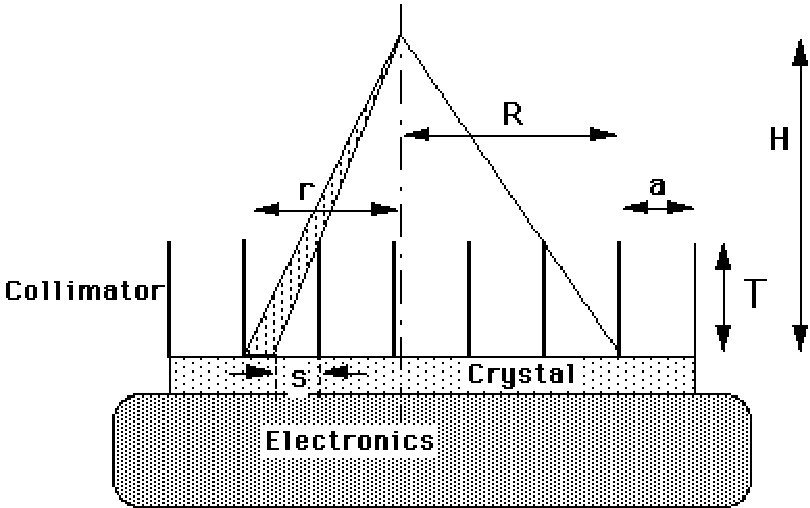
\includegraphics[width=0.5\textwidth]{figs/fig_collimator_calc.pdf}
\caption{\emph{Parallel hole collimator.}}
\label{fig:collimator_calc}
\end{figure}

Fig. \ref{fig:collimator_calc} shows the cross section of a parallel
hole collimator with septa length $T$ and septa spacing $a$. At a
distance of $H$, a radioactive point source is located.  If the
collimator would really absorb all photons except those propagating
exactly perpendicular to the detector, then the image would be a
point.  However, fig. \ref{fig:collimator_calc} shows that photons
propagating along slightly inclined lines may also reach the detector.
Therefore the image will not be a point. Because the image of a point
is characteristic for the system, such images are often studied. By
definition, the image of a point is the {\em point spread function}
(PSF) of the imaging system. 

Assume that the thickness of the septa can be ignored, that $H$ is large
compared to the length of the septa $T$, and that $T$ is large compared to
$a$.  We will also ignore septal penetration (i.e. gamma-photons traveling
through the septa instead of getting absorbed). The light (e.g. 140 keV
photons) emitted by the source makes the septa cast a shadow on the detector
surface. In fact, most of the detector is in that shadow, except for a small
region facing the source. We will regard the center of that region,
immediately under the source, as the origin of the detector plane. The length
of the shadow $s$ cast by a septum on the detector is then
\begin{equation}
s = r \frac{T}{H}
\end{equation}
where $r$ is the distance to the origin. The fraction of the detector element
that is actually detecting photons is
\begin{equation}
f = \frac{a - s}{a} = 1 -  \frac{r T}{a H} = 1 - \frac{r}{R} \label{eq:collim:fraction}
\end{equation}
This expression holds for $r$ between 0 and $R$, where $R$ is the
position at which the shadow completely covers the detector so that $f
= 0$. The expression gives the fraction of the photons detected at
$r$, relative to the number that would be detected at the same
position if there was no collimator. This latter number is easy to
compute. The source is emitting photons uniformly, so the number of
photons per solid angle is constant. Stated otherwise, if we would put
a point source in the center of a spherical uncollimated detector with
radius $H$, the detector surface would be uniformly irradiated. The
total area of the sphere is $4 \pi H^2$, so the sensitivity per unit
area is $1 / (4 \pi H^2)$. Multiplying with the collimator sensitivity
produces the point spread function of the collimated detector at
distance $H$:
\begin{equation}
\mbox{PSF}(r) = (1 -  \frac{r T}{a H}) \frac{1}{4 \pi H^2}
  \label{eq:collim:psf}
\end{equation}
In this expression, we have ignored the fact that for a flat detector, the
distance to the point increases with $r$. The approximation is fair if $r$ is
much smaller than $H$. Consequently, the PSF has a triangular profile, as
illustrated in figure \ref{fig:collimatorpsf}.

To calculate (approximately) the total collimator sensitivity, expression
(\ref{eq:collim:psf}) must be integrated over the region where PSF$(r)$ is
non-zero. We assume circular symmetry and use integration instead of the
summation (actually required by the discrete nature of the problem).
Integration assumes that $a$ and $T$ are infinitely small. Since we use only
the ratio, this poses no problems.
%
\begin{align}
\mbox{sens} &= \frac{1}{4 \pi H^2}
                  \int_0^R (1 - \frac{r T}{a H}) 2 \pi r dr \nonumber \\
            &= \frac{1}{4 \pi H^2}\frac{\pi R^2}{3}
             = \frac{1}{12} \left( \frac{a}{T} \right)^2
    \label{eq:collim:sens}\\
R & = & \frac{a H}{T} 
\label{eq:collim:fwhm}
\end{align}
%
Note that a similar result is obtained if one assumes that the
collimator consists of square grid of square holes. One finds:
\begin{equation}
\mbox{sens} \;\; = \;\;  \frac{1}{4 \pi H^2} 
  \int_{-R}^{R} dx \int_{-R}^{R} dy (1 - \frac{|x|}{R}) \; (1 -
  \frac{|y|}{R})
  \;\; = \;\; \frac{1}{4 \pi} \left( \frac{a}{T} \right)^2.
\end{equation}
In reality, the holes are usually hexagonal. With a septa length of 2
cm and septa spacing of 1 mm, about 1 in 5000 photons is passing
through the collimator, according to equation
(\ref{eq:collim:sens}). It is fortunate that the sensitivity does not
depend on the distance $H$.


It is easy to show that (\ref{eq:collim:fwhm}) is also equal to the FWHM of the
PSF: you can verify by computing the FWHM from (\ref{eq:collim:psf}). So the
FWHM of the spatial resolution {\em increases linearly with the distance to
the collimator!}  Therefore, the collimator must always be as close as
possible to the patient, and failure to do so leads to important image
degradation! Many gamma cameras have hardware to automically minimize
the distance between patient and collimator during scanning.

To improve the resolution, the ratio $a/T$ must be decreased. However, the
sensitivity is proportional to the square of $a/T$. As a result, the
collimator must be a compromise between high sensitivity and low FWHM.

The PSF is an important characteristic of the linear system, which allows us
to predict how the system will react to any input. See appendix
\ref{app:convolution} if you are not familiar with the concept of PSF and
convolution integrals.

In section \ref{sec:resolution} we have seen that the {\em intrinsic
resolution} of a typical scintillation detector has a FWHM of about 4 mm. Now,
we have seen that the collimator contributes significantly to the FWHM, but in
the derivation, we have ignored the intrinsic resolution.  Obviously, they
have to be combined to obtain realistic results, so we must ``superimpose'' the
two random processes. The probability distribution of each random process is
described as a PSF. To compute the overall probability distribution, the
second PSF must be ``applied'' to every point of the first
one. Mathematically, this means that the two PSFs must be convolved. If we
make the reasonable assumption that the PSFs are Gaussian, convolution
becomes very simple, as shown in appendix \ref{app:convol2gauss}: the result
is again a Gaussian, and its variance equals the sum of variances of the
contributing Gaussians.

At distances larger than a few cm, the collimator PSF dominates the spatial
resolution. The PSF increases in the order of half a cm per 10 cm distance,
but there is a wide range: different types of collimator exist, either
focusing on resolution or on sensitivity.

%
\begin{figure}[tb]
\centering
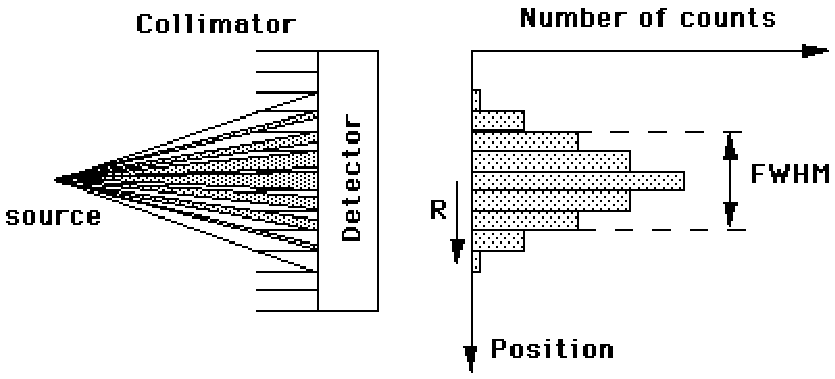
\includegraphics[width=0.5\textwidth]{figs/fig_collimatorpsf.pdf}
\caption{\label{fig:collimatorpsf} \emph{Point spread function of
          the collimator. The number of detected photons at a point in the
          detector decreases linearly with the distance $r$ to the central
          point.}}
\end{figure}

In the calculations above, the thickness of the septa has been
ignored. In reality, the septa have to be thick enough to stop the
photons hitting them. Septa are made from high-Z materials, like lead
or tungsten, to maximize the photon attenuation. High resolution
collimators are optimized for imaging with \textsuperscript{99m}Tc: the septa are
relatively thin, and $a/T$ is small, resulting in high resolution but
not so high sensitivity. High sensitivity collimators have a larger
$a/T$, producing poorer resolution. High energy collimators are
designed for isotopes emitting high energy photons, such as $^{131}$I
(see table \ref{tab:rntisotopes}). They have thicker septa to
minimize the number of photons penetrating them. To account for
the septa thickness, equation (\ref{eq:collim:sens}) can be extended
to
\begin{equation}
  \mbox{sens} =  \frac{1}{12} \left( \frac{a}{T} \right)^2
                 \;\frac{a^2}{(a+s)^2}
\end{equation}
where $a$ is the distance between neighboring septa and $s$ is the septa
thickness. Using thicker septa while keeping the resolution reduces
the collimator sensitivity.


\subsection{Electronic and mechanical collimation in the PET camera} \label{sec:petcollim}
%===================================================================
\subsubsection{Electronic collimation: coincidence detection}
%------------------------------------
During positron annihilation, two photons are emitted in opposite
directions. If both are detected, we know that the annihilation occurred
somewhere on the line connecting the two detectors. So in contrast to SPECT,
no mechanical collimator is needed. However, we need fast electronics, since
the only way to test if two detected photons could belong together, is by
checking if they have been emitted simultaneously.

We first consider a single detector pair as shown in figure
\ref{fig:petdetectorpair}, and study its characteristics by computing its
response to a point source. The detector has a square surface of size $d$, and
the distance between the detectors is $2R$. We choose the origin in the point of
symmetry, and see how the response changes if we change the position of the
point source. Keep in mind that an event is only valid if both photons of the
photon pair are detected.
%
\begin{figure}[tb]
\centering
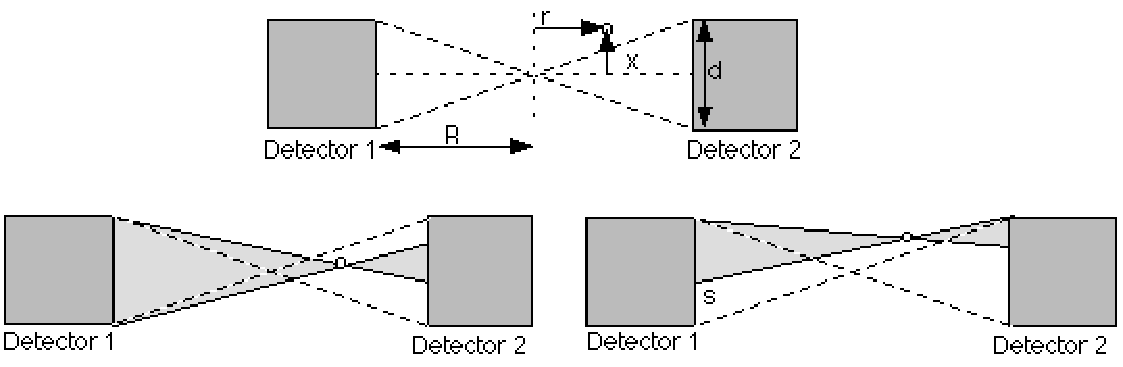
\includegraphics[width=0.9\textwidth]{figs/fig_petdetectorpair.pdf}
\caption{\label{fig:petdetectorpair} \emph{A point source positioned in the
field of view of a pair of detectors}}.
\end{figure}

Assume that the point source is moved along the $r$-axis: $x = 0$. Then the
limiting detector is the far one: if one photon reaches the far detector, the
other photon will surely reach the other detector. The number of detected
photon pairs is proportional to the solid angle occupied by the two detectors:
\begin{equation}
  \mbox{PSF}(x=0, r) = \frac{2 d^2}{4 \pi (R+r)^2} = \frac{d^2}{2 \pi (R+r)^2}
\end{equation}
This is an approximation: we assume that the far detector surface coincides
with the surface of a sphere of radius $R+r$. It does not, because it is flat.
However, because $d$ is very small compared to $R$, the approximation is very
good.

We now move the point source vertically over a distance $x$. As long as the
point is between the dashed lines in figure \ref{fig:petdetectorpair}, nothing
changes (that is, if we ignore the small decrease in solid angle due to the
fact that the detector surface is now slightly tilted when viewed from the
point source). However, when the point crosses the dashed line, the far
detector is no longer fully irradiated. A part of the detector surface no
longer contributes: if a photon reaches that part, the other photon will miss
the other detector. The height $s$ is computed from simple geometry (figure
\ref{fig:petdetectorpair}):
\begin{equation}
  s(x) = \left( |x| - \frac{d |r|}{2 R} \right) \frac{2R}{R-|r|}
\end{equation}
The first factor is the distance between the point and the dashed line, the
second factor is the magnification due to projection of that distance to the
far detector. This equation is only valid when $d r / (2R) \leq x \leq
d/2$. Otherwise, $s = 0$ if $x$ is smaller than $dr/(2R)$, and $s = d$ if $x$
is larger. In the center, $r = 0$ and we have simply that $s(x) = 2 |x|$.
Knowing the active detector area, we can immediately compute the
corresponding solid angle to obtain the detector pair sensitivity as a
function of the point source position (which can be regarded as a PSF):
\begin{equation}
 \mbox{PSF}(x, r) = \frac{(d - s(x)) d}{2 \pi (R+|r|)^2}
\end{equation}
We can move the point also in the third dimension, which we will call $y$. The
effect is identical to that of changing $x$, so we obtain:
\begin{equation}
 \mbox{PSF}(x, y, r) = \frac{(d - s(x)) (d - s(y))}{2 \pi (R+|r|)^2}
\end{equation}

From these equations it follows that the PSF is triangular in the center,
rectangular close to the detectors and trapezoidal in between.  Introducing
that third dimension, we obtain for the PSF in the center and close to the
detector respectively:
\begin{align}
  \mbox{PSF}(x, y, 0) &= \frac{(d - 2|x|)(d - 2 |y|)}{2 \pi R^2}\\
  \mbox{PSF}(x, y, R) &= \frac{d^2}{8 \pi R^2}
\end{align}
We can compute the average sensitivity within the field of view by integrating
the PSF over the detector area $x \in [-d/2, d/2], y \in [-d/2,
d/2]$ and divide by $d^2$. It is simple to verify that in both cases we obtain:
\begin{equation}
  \mbox{sens} = \frac{d^2}{8 \pi R^2} \label{eq:pet_totsens}
\end{equation}
showing that sensitivity is independent of position in the detection plane, if
the object is large compared to $d$.

Finally, we can estimate the sensitivity of a complete PET system consisting
of a detector ring with thickness $d$ and radius $R$, assuming that we have a
positron emitting source near the center of the ring. We assume that the ring
is in the $(y,r)$-plane, so the $x$-axis is the symmetry axis of the detector
ring.  One approach is to divide the detector area by the area of a sphere
with radius $R$, as we have done before. This yields:
\begin{equation}
  \mbox{PETsens}_{x=0} = \frac{2 \pi d R}{ 4 \pi R^2} = \frac{d}{2R}
\end{equation}
This is the maximum sensitivity, obtained for $x = 0$. The average over $ =
-d/2 \ldots d/2$ is half that value, since in the center of the PET, the
sensitivity varies linearly between the maximum and zero:
\begin{equation}
  \mbox{PETsens} = \frac{d}{4R}. \label{eq:petsens}
\end{equation}

\subsubsection{Resolution of coincidence detection}
%------------------------------------
Until now, we have always assumed that annihilation takes place very close to
the emission point, and that the photons are emitted in exactly opposite
directions. In reality, there are small deviations, which limit the
theoretical resolution of PET. 

\begin{table}
\caption{Maximum and mean kinetic energy (k.e.), maximum and mean path length
of the positron for the most common PET isotopes.}
\label{tab:positron_length}
\begin{center}
\begin{tabular}{|c|c|c|c|c|}
\hline
Isotope   & Max k.e. [MeV] & mean k.e. [MeV] & Max path [mm] & Mean path [mm]\\
\hline
$^{11}$C  & 0.96 & 0.39 & 3.9    & 1.1 \\
$^{13}$N  & 1.19 & 0.49 & 5.1    & 1.5 \\
$^{15}$O  & 1.72 & 0.73 & 8.0    & 2.5 \\
$^{18}$F  & 0.64 & 0.25 & 2.4    & 0.6 \\
$^{68}$Ga & 1.90 & 0.85 & 8.9    & 2.9 \\
$^{82}$Rb & 3.35 & 1.47 & 17     & 5.9 \\
\hline
\end{tabular}
\end{center}
\end{table}

As shown in table \ref{tab:positron_length}, the path depends on the
kinetic energy of the positron. The positron can only annihilate if
its kinetic energy is sufficiently low, so if it is emitted at high
speed, it will travel ``far'' (up to a few mm). During its trajectory,
it dissipates its energy in collisions with surrounding electrons. The
mean path length (positron range) of $^{18}$F is small and has a very
limited effect on the spatial resolution. For some other isotopes,
like $^{68}$Ga and $^{82}$Rb, the positron range is several mm.

Momentum is preserved during annihilation, so the momentum of both photons
must equal the momentum of the positron and the electron. This momentum is
usually not zero, so the photons cannot be emitted in exactly opposite
directions (the momentum of a photon is a vector with amplitude $h/\lambda$
and pointing in the direction of propagation). As shown in figure
\ref{fig:positron_error}, there is a deviation of about 0.5\textdegree, which
corresponds to a 2.0 mm offset for a detector ring with 80 cm diameter.
%
\begin{figure}[tb]
\centering
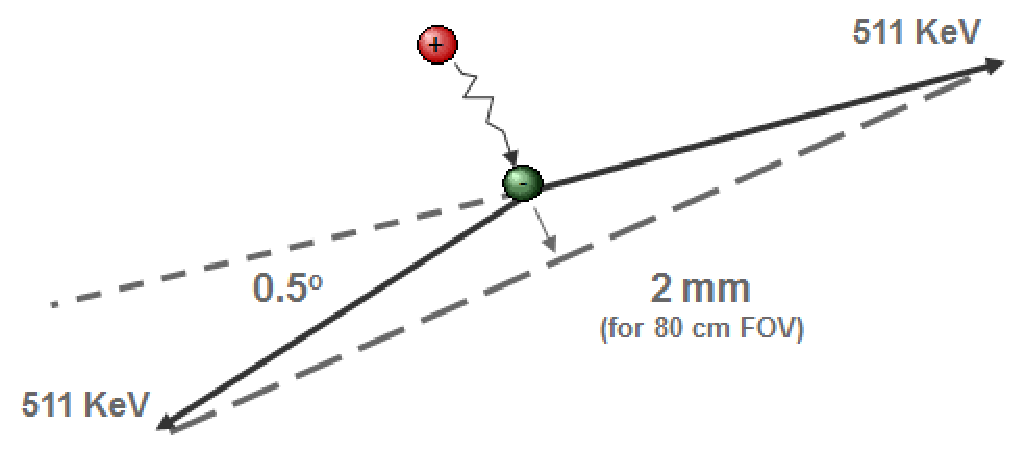
\includegraphics[width=0.5\textwidth]{figs/fig_positron_error.pdf}
\caption{\label{fig:positron_error} \emph{The distance traveled by the
positron and the deviation from 180 degrees in the angle between the photon
paths limit the best achievable resolution in PET}}.
\end{figure}


\begin{figure}[tb]
\centering
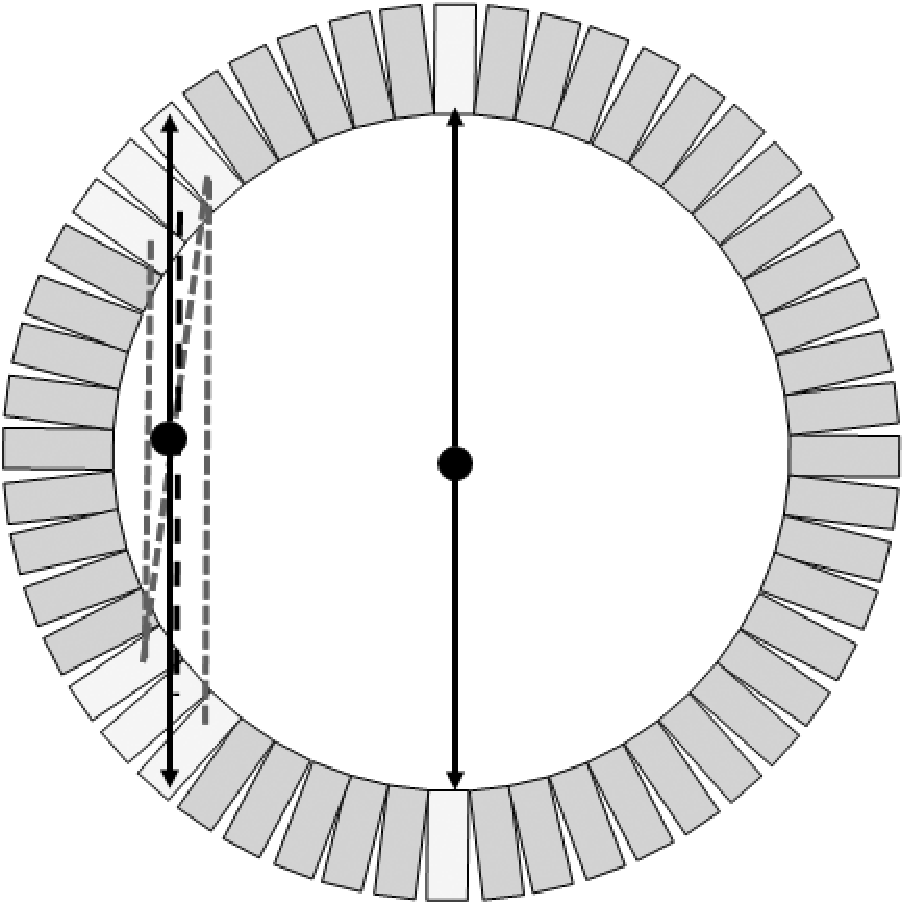
\includegraphics[width=0.3\textwidth]{figs/fig_doi.pdf}
\caption{\label{fig:doi} \emph{Resolution loss as a result of
    uncertainty about the depth of interaction}}.
\end{figure}
%
The resolution is further degraded by the unknown ``depth of
interaction'' of the photon inside the crystal. As shown in figure
\ref{fig:doi}, photons emitted near the edge of the field of view
might traverse one crystal to scintillate only in the next
one. Because we don't know where in the crystal the scintillation took
place, we always have to assign a fixed depth of interaction to the
event. The mispositioning of these events causes a loss of resolution
that increases with the distance from the center. PET systems have
been designed and built that can measure the depth of interaction to
reduce this loss of resolution.


\subsubsection{Mechanical collimation: inter-plane septa} \label{sec:septa}
%------------------------------------
In the previous section we have seen why a PET-camera does not need a
collimator. We also know that the PET-camera can only measure photon pairs
originating somewhere within the detection plane. However, photons coming from
radioactivity outside that plane could also reach the detectors, and produce
undesired scintillations, which provide no information, or even worse, wrong
information. Therefore, it is useful to shield the detector ring against
photons coming from outside the field of view. This is done with so-called
septa, as shown in figure \ref{fig:pet_septa}. The septa provide some
collimation in the direction perpendicular to the detection plane, but there is
no collimation within the plane. The septa reduce the number of single
photons, scattered photons, random coincidences and triple (or more)
coincidences.

%
\begin{figure}[tb]
\centering
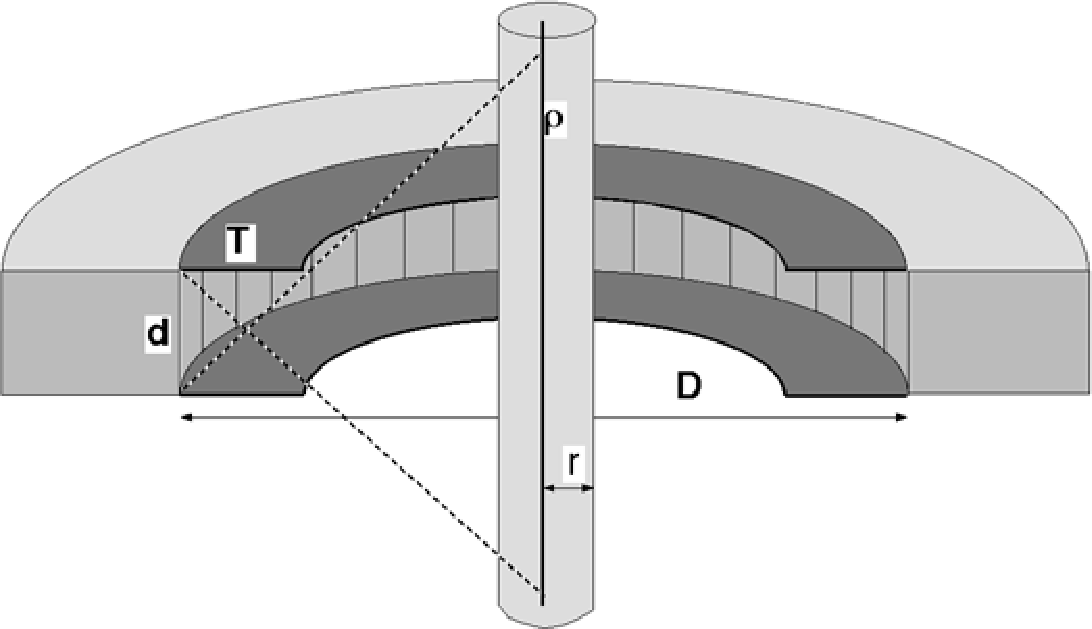
\includegraphics[width=0.5\textwidth]{figs/fig_pet_septa.pdf}
\caption{\label{fig:pet_septa} \emph{A PET ring detector (cut in half) with a
cylindrical homogeneous object, containing a radioactive wire near the
symmetry axis}}.
\end{figure}

Before these events are described, we have to better define what is meant with
a coincidence. Two photons are detected {\em simultaneously} if the difference
in detection times is lower than a predefined threshold, the ``time window''
of the PET-system. The time window cannot be arbitrarily short for the
following reasons:
\begin{itemize}
  \item The time resolution of the electronics is limited: electricity is
        never faster than light, and it is delayed in every electronical
        component.  Of course, we do not want to reject true coincidences
        because of errors in timing computation.
  \item The diameter of the PET-camera is typically about 1 m for a
        whole body system, and about half that for a brain
        system. Light travels about 1 m in 3 ns. Consequently, the
        time window should not be below 3 ns for a 1 m diameter
        system.
\end{itemize}
For these reasons, current systems use a time window of about 5 to 10
ns. Recently, PET systems have been built with a time resolution
better than 1 ns. With those systems, one can measure the difference
in arrival time between the two photons and deduce some position
information from it. This will be discussed in section \ref{sec:TOF}.

Figure \ref{fig:pet_random_enzo} shows the difference between a true
coincidence, which provides valuable information, and several other events
which are disturbing or even misleading. A single event provides no
information and is harmless. But if two single events are simultaneous (random
coincidence), they are indistinguishable from a true coincidence. If one (or
both) of the photons is scattered, the coincidence provides wrong information:
the decaying atom is not located on the line connecting the two
detectors. Finally, a single event may be simultaneous with a true
coincidence. Since there is no way to find out which of the three photons is
the single one, the entire event is ignored and information is lost.

\begin{figure}[tb]
\centering
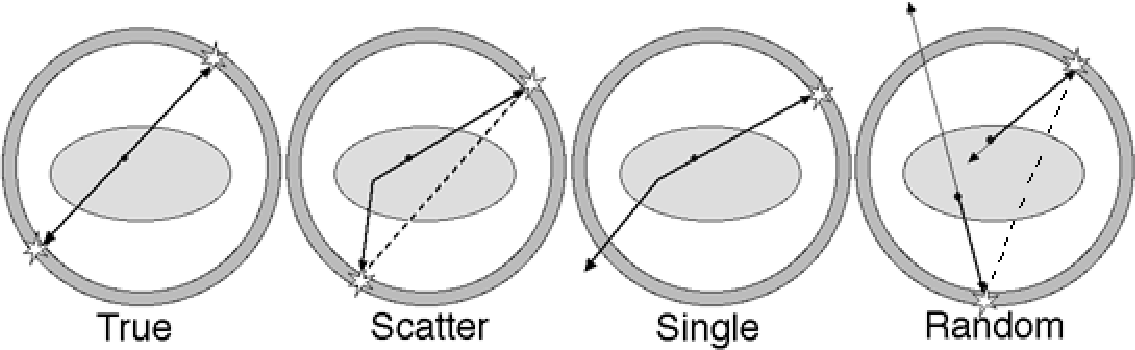
\includegraphics[width=0.9\textwidth]{figs/fig_pet_random_enzo.pdf}
\caption{\label{fig:pet_random_enzo} \emph{True coincidence, scattered
coincidence, single event, random coincidence}}.
\end{figure}

To see how the septa dimensions influence the relative contribution of the
various possible events, some simple computations can be carried out using the
geometry shown in figure \ref{fig:pet_septa}. Assume that we have a
cylindrical object in the PET-camera. In the center of the cylinder, there is
a radioactive wire, with activity $\rho$ per unit length. The cylinder has
radius $r$ and attenuation coefficient $\mu$. This object represents an
idealized patient: there is activity, attenuation and Compton scatter in the
attenuating object as in a patient; the unrealistic choice of dimensions makes
the computations easier. The PET-camera diameter is $D$, the detector size is
$d$ and the septa have length $T$. The duration of the time window is
$\tau$. Finally, we assume that the detector efficiency is $\epsilon$, which
means that if a photon reaches the detector, it has a chance of $\epsilon$ to
produce a valid scintillation, and a chance of $1 - \epsilon$ to remain
undetected.\\[2mm]

To compute the number of {\bf true coincidences} per unit of time, we must
keep in mind that both photons must be detected, but that their paths are not
independent. To take into account the influence of the time window, it helps
to consider first a short time interval equal to the time window $\tau$. After
that, we convert the result to counts per unit of time by dividing by
$\tau$. Why we do this will become clear when dealing with randoms. We proceed
as follows:
\begin{itemize}
%
\item The activity in the field of view is $\rho d$. 
%
\item Both photons can be attenuated, the attenuated activity is $\rho d a^2$,
with $a = \exp(-\mu r)$.
%
\item As we have derived above (see eq (\ref{eq:petsens})), the
geometrical sensitivity is $d/(2D)$.
%
\item Both photons must be detected if they hit the detectors, so the
effective sensitivity is $\epsilon^2 d / (2D)$.
%
\item The probability that a photon will be seen is proportional to the
      scan time $\tau$.
%
\item To compute the number of counts per time unit, we multiply with $1/\tau$.
\end{itemize}
We only care about the influence of the design parameters, so we ignore all
constants. This leads to:
\begin{equation}
  \mbox{trues} \sim \rho a^2 \epsilon^2 \frac{d^2}{D} \label{eq:pet_trues}
\end{equation}

For {\bf scatters} the situation is very similar, except for two
issues: (1) the probability for a scatter event to occur depends on the
attenuating material and (2), the combined photon path is not a
straight line but a broken one.

Consider a source with activity $\lambda$ emitting photons at $x = 0$
along the $x$-axis, in a material met linear attenuation coefficient
$\mu$ that covers the interval $x \in [-r, r]$. Then the probability
of a photon arriving at $x$ is proportional to $\lambda e^{- \mu x}$,
and the probability that it scatters there is proportional to $\lambda
e^{- \mu x} \mu \; dx$. The probability that this scattered photon will
not be attenuated is determined by how much material it is propagating
through, and can be roughly estimated as $e^{\mu(r-x)}$. To obtain all
scattered photons leaving the object we integrate this from the source
position to the boundary of the material: 
\begin{equation}
  \lambda \int_0^r e^{-\mu x} \mu \; e^{-\mu(r - x)} dx \;\;\;
  = \;\; \lambda e^{-\mu r} \mu r \;\;
  = \;\; \lambda a \mu r,
\end{equation}
where the last equation is obtained by setting $e^{-\mu r} = a$.

The other issue is that the combined photon path is a broken
line. This has two consequences. First, the field of view is larger
than for the trues. Second, the path of the second photon is (nearly)
independent of that of the first one.

We will assume that only one of the photons undergoes a single Compton scatter
event, so the path contains only a single break point. The corresponding field
of view is indicated with the dashed line in figure \ref{fig:pet_septa}. The
length of the wire in the field of view is then $d (D-T) / T$, but since $T$ is
much smaller than $D$ we approximate it as $d D/T$.

Each of the photons goes its own way. This will only lead to detection if both
happen to end up on a detector and are detected. For each of them, that
probability is proportional to $\epsilon d / D$, so for the pair the detection
probability is $(\epsilon d / D)^2$. For the trues this factor was not
squared, because detection of one photon guarantees detection of the other!

Attenuation of scattered photons is complex, since they have lower energy and
travel along oblique lines. However, if we assume that the septa are not too
short and that the energy resolution is not too bad, we can ignore all that
without making too dramatic an error. (We only want to see the major
dependencies, so we can live with moderately dramatic errors.)
Consequently, we have for the scatters count rate
\begin{equation}
  \mbox{scatters} \;\;\sim\;\; \rho d \frac{D}{T} \; \mu r \; a^2
     \; \left( \frac{\epsilon d}{D} \right)^2
  \;\;=\;\;  \rho \mu r a^2 \epsilon^2 \frac{d^3}{DT}
       \label{eq:pet_scatters}
\end{equation}

A {\bf single}, non-scattered photon travels along a straight line, so the
singles field of view is the same as that of the scatters, and the
contributing activity is $\rho d D / T$. The attenuation is $a$. The effective
sensitivity is proportional to $\epsilon d / D$. The number of singles in a
time $\tau$ is proportional to $\tau$. Finally, we divide by $\tau$ to obtain
the number of single events per unit of time. This yields:
\begin{equation}
  \mbox{singles} \sim \rho a \epsilon \frac{d^2}{T} \label{eq:pet_singles}
\end{equation}

A {\bf random coincidence} consists of two singles, arriving {\em
simultaneously}. So if we study a short time interval $\tau$ equal to the time
window, we must simply multiply the probabilities of the two singles, since
they are entirely independent of each other. Afterwards, we multiply with
$1/\tau$ to compute the number of counts per time unit. So we obtain:
\begin{equation}
  \mbox{randoms} \sim \rho^2 a^2 \epsilon^2 \frac{d^4}{T^2} \tau
      \label{eq:pet_randoms}
\end{equation}

Similarly, we can compute the probability of a ``{\bf triple coincidence}'',
resulting from simultaneous detection of a true coincidence and a single
event. This produces:
\begin{equation}
  \mbox{true + single} \sim \rho^2 a^3 \epsilon^3 \frac{d^4}{TD} \tau
\end{equation}

As you can see, the trues count rate is not affected by either $\tau$
nor $T$, in contrast to the unwanted events. Consequently, we want
$\tau$ to be as short as possible to reduce the randoms and triples
count rate. We have seen that for current systems this is about 10 ns
or even less. Similarly, we want $T$ to be as large as possible to
reduce all unwanted events. Obviously, we need to leave some room for
the patient.


\subsubsection{2D and 3D PET} \label{sec:2D3DPET}
%------------------------------------
In the previous paragraphs we have studied a single ring of PET
detectors, and we have shown that shielding the detectors with septa
reduces the scatter and random coincidence rate, without affecting the
true coincidence rate. In current clinical systems, multiple rings are
combined in a single device, as shown in figure \ref{fig:jnpet}. In
the past, many of these systems could be operated in two modes.  In
2D-mode, the rings are separated by septa. In 3D-mode, the septa are
retracted, only the shielding at the edges of the axial field of view
remain. Current PET systems have no septa between the detector rings,
they are always operated in 3D mode.

\begin{figure}[tb]
\centering
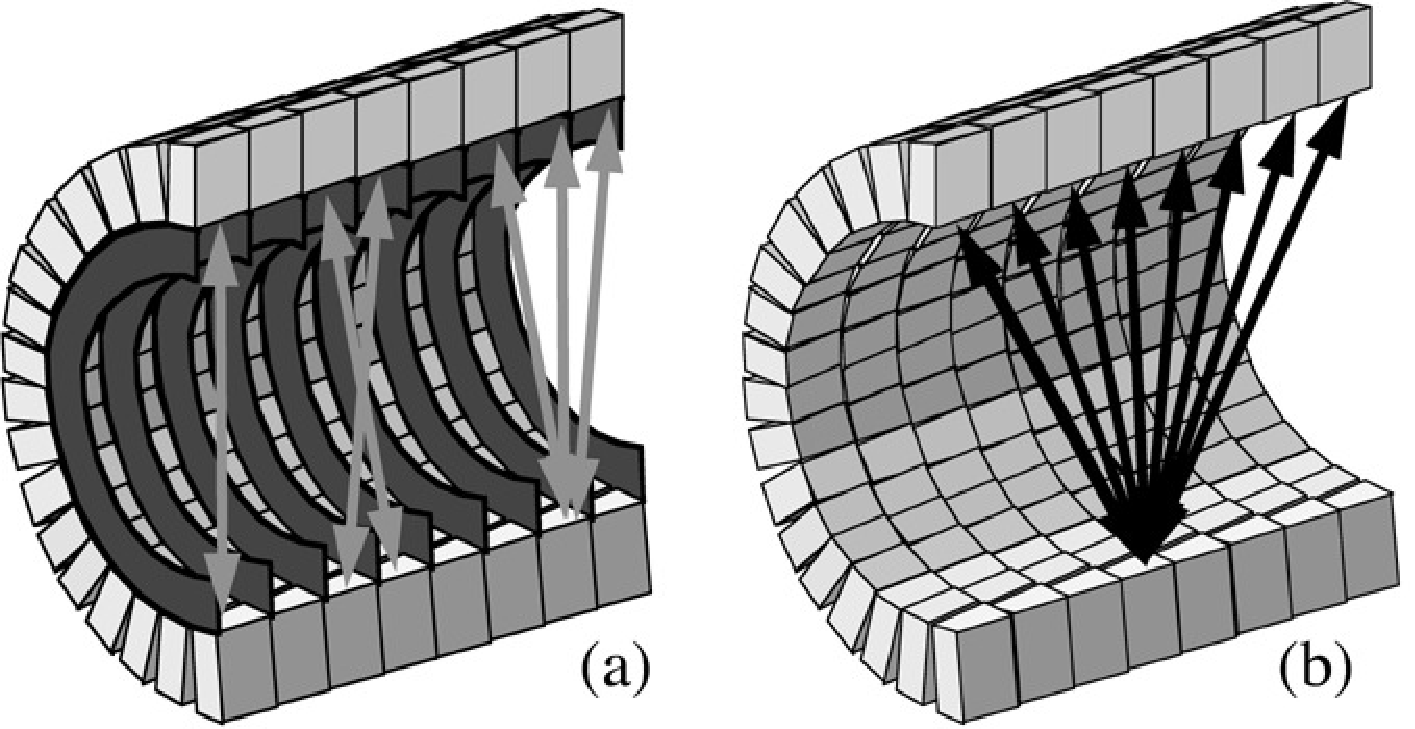
\includegraphics[width=0.5\textwidth]{figs/fig_jnpet.pdf}
\caption{\label{fig:jnpet} \emph{Positron emission tomograph (cut in
half). When septa are in the field of view (a), the camera can be regarded as
a series of separate 2D systems. Coincidences along oblique projection lines
between neighboring rings can be treated as parallel projection lines from an
intermediate plane. This doubles axial sampling: 15 planes are reconstructed
from 8 rings. Retracting the septa (b), increases the number of projection
lines and hence the sensitivity of the system, but fully 3D reconstruction is
required.}}
\end{figure}

In 2D mode, there are two types of planes: direct planes, located in the
center of the ring, and cross-planes, located between two neighboring
rings. The direct planes correspond to what we have seen above for a single
ring system. A photon pair belongs to a cross plane if one photon is detected
in ring $i$ and the other one in ring $i+1$. The small inclination of the
projection line can be ignored, and such coincidences are processed as if they
were acquired by an imaginary detector ring located at $i + 0.5$. This
improves axial sampling. It turns out that the cross-planes are in fact
superior to the direct planes: near the center the axial resolution is
slightly better because of the shadow cast by the septa on the contributing
detectors, and the sensitivity is nearly twice that of direct planes because
of the larger solid angle.

According to the Nyquist criterion, the sampling distance should not be longer
than half the period of the highest special frequency component in the
acquired signal (you need at least two samples per period to represent a sine
correctly). Without the cross-planes, the criterion would be violated. So the
cross-planes are not only useful to increase sensitivity, the are needed to
avoid aliasing as well.\\[2mm]

In 3D mode, the septa are retracted, except for the first and last one. The
detection is no longer restricted to parallel planes, photon pairs traveling
along oblique lines are now accepted as well. In chapter
\ref{ch:image_formation} we will see that this has a strong impact on image
reconstruction.

This has no effect on spatial resolution, since that is determined by
the detector size. But the impact on sensitivity is very high. In fact,
we have already computed all the sensitivities in section
\ref{sec:septa}. Those expressions are still valid for 3D PET, if we
replace $d$ (the distance between the septa) with $Nd$, where $N$ is
the number of neighboring detector rings. To see the improvement for
3D mode, you have to compare to a concatenation of $N$ independent
detector rings (2D mode), which are $N$ times more sensitive than a
single ring (at least if we wish to scan an axial range larger than
that seen by a single ring). So you can see that the sensitivity for
trues increases with a factor of $N$ when going from 2D to
3D. However, scatters increase with $N^2$ and randoms even with
$N^3$. Because the 3D PET is more sensitive, we can decrease the
injected dose with a factor of $N$ (preserving the count rate). If we
do that, randoms will only increase with $N^2$. Consequently, the
price we pay for increased sensitivity is an even larger increase of
disturbing events. So scatter and randoms correction will be more
important in 3D PET than in 2D PET. It turns out that scatter in
particular poses problems: it was usually ignored in 2D PET, but this
is no longer acceptable in 3D PET. Various scatter correction
algorithms for 3D PET have been proposed in the literature, the one
mostly used is described below (\ref{sec:petscatcor}).

\section{Partial volume effect} \label{sec:pv}
%%%%%%%%%%%%%%%%%%%%%%%%%%%%%%%%%%%%%%%%%
\begin{figure}[tb]
\centering
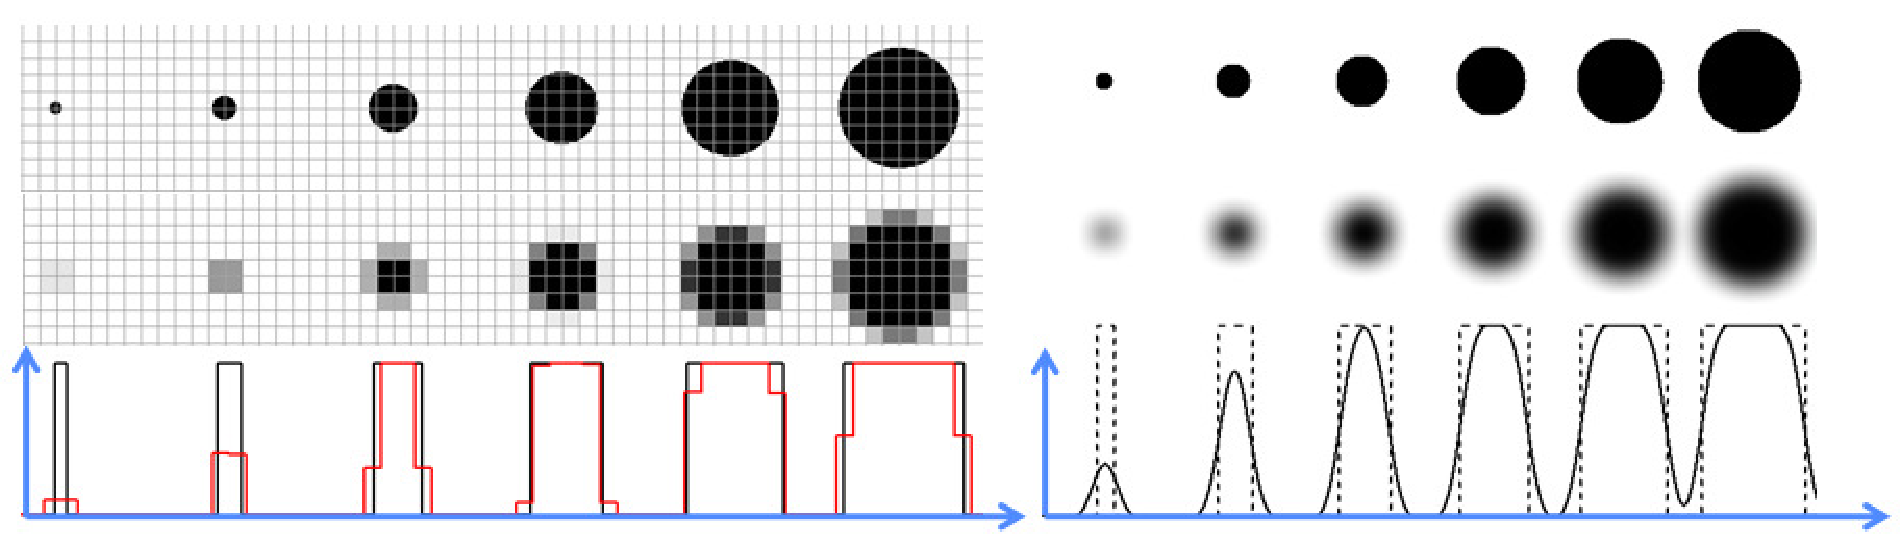
\includegraphics[width=0.9\textwidth]{figs/fig_pv.pdf}
\caption{\label{fig:pv} \emph{The partial volume effect caused by the
finite pixel size (left), and by the finite system PSF (right). The
first row shows the true objects, the second row illustrates the
partial volume effect due to pixels and PSF, and the last row compares
horizontal profiles to the true objects and the images.  Objects that
are small compared to the pixel size and/or the PSF are poorly
represented.}}
\end{figure}
%
As explained above, resolution is not the strongest point of nuclear
medicine. Other medical imaging systems (CT, MR, ultrasound) have a
much better resolution. One often uses the term {\em partial volume
effect} to refer to problems caused by poor resolution. The idea is
that if an object only fills part of a pixel, the pixel contains two
things: object and background. Because the pixel has only one value,
it does not give a reliable representation of either. Figure
\ref{fig:pv} illustrates this for a disk imaged with some imaging
system. If the object is large compared to the pixels of the image,
then the image gives a good representation of the object. However,
small objects are poorly represented. As can be seen in the profiles,
the maximum value in the image is much smaller than the true maximum
intensity of the object. The obvious remedy is to use sufficiently
small pixels.

However, if the pixels are small, the imaging performance is limited
by the system point spread function, as illustrated in the second
panel of figure \ref{fig:pv}. The image can be regarded as a
convolution of the true intensities with the PSF. The effect is very
similar as that of the big pixels, one could say that the object only
partially fills the PSF. Again, the maximum intensity of small objects
is severely underestimated, and their size is overestimated.

Consequently, nuclear medicine imaging systems tend to underestimate
the maximum intensity and overestimate the size of small objects. The
{\em recovery coefficient} is the ratio of the estimated and true
maximum. The so-called {\em spill over} is the amount of apparent
activity showing up outside the true object boundaries due to the
blurring.

\section{Compton scatter correction} \label{sec:scatter}
%%%%%%%%%%%%%%%%%%%%%%%%%%%%%%%%%%%%%%%%%
% Scatter in SPECT, evt meerdere energieen.
% Pile-up
%----
\subsection{Gamma camera} \label{sec:spectscatcor}
%------------------------
Compton scatter causes photons to be deviated from their original trajectory,
and to propagate with reduced energy along a new path. Consequently, photons
with reduced energy can reach the detector via a broken line. Such photons are
harmful: they provide no useful information and produce an unwanted
inhomogeneous background in the acquired images (fig
\ref{fig:scatter_gammacamera}).

\begin{figure}[tb]
\centering
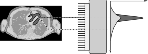
\includegraphics[width=0.5\textwidth]{figs/fig_scatter_gammacamera.pdf}
\caption{\label{fig:scatter_gammacamera} \emph{Compton scatter allows
photons to reach the camera via a broken line. These photons produce a smooth
background in the acquired projection data.}}
\end{figure}

We have seen in section \ref{sec:compton_scatter} that the photon loses more
energy for larger scatter angles. The gamma camera (or the PET camera) measures
the energy of the photon, so it can reject the photon if its energy is low.

However, if the energy loss during Compton scatter is smaller than or
comparable to the energy resolution of the gamma camera, then it may
survive the energy test and get accepted by the camera. Figure
\ref{fig:scatter_spectrum} shows the energy spectrum as measured by
the gamma camera. A Monte Carlo simulation was carried out as well,
and the resulting spectrum is very similar to the measured one. The
simulation allows to compute the contribution of unscattered (or
primary) photons, photons that scattered once and photons that
suffered multiple scatter events. If the energy resolution were
perfect, the primary photon peak would be infinitely narrow and all
scattered photons could be rejected. But with a realistic energy
resolution the spectra overlap, and acceptance of scattered photons is
unavoidable.

\begin{figure}[tb]
\centering
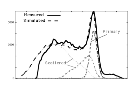
\includegraphics[width=0.5\textwidth]{figs/fig_scatter_spectrum.pdf}
\caption{\label{fig:scatter_spectrum} \emph{The energy spectrum measured by
the gamma camera, with a simulation in overlay. The simulation allows to
compute the spectrum of non-scattered (primary) photons, single scatters and
multiple scatters. The true primary spectrum is very narrow, the measured one
is widened by the limited energy resolution.}}
\end{figure}

Figure \ref{fig:scatter_spectrum} shows a deviation between simulation and
measurement for high energies. In the measurement it happens that two photons
arrive simultaneously. If that occurs, the gamma camera adds their energies
and averages their position, producing a mispositioned count with high
energy. Such photons must be rejected as well. The simulator assumed
that each photon was measured independently. The simulator deviates also at
low energies from the measured spectrum, because the camera has not recorded
these low-energy photons.

To reject as much as possible the unwanted photons, a narrow energy
window is centered around the tracer energy peak, and all photons with
energy outside that window are rejected. Current gamma cameras can use
multiple energy windows simultaneously. That allows us to administer
two or more different tracers to the patient at the same time, if we
make sure that each tracer emits photons at a different energy. The
gamma camera separates the photons based on their energy and produces
a different image for each tracer. For example, $^{201}$Tl emits
photons of about 70 keV (with a frequency of 0.70 per desintegration)
and 80 keV (0.27 per desintegration), while \textsuperscript{99m}Tc\ emits photons
of about 140 keV (0.9 per desintegration). $^{201}$Tl labeled thallium
chloride can be used as a tracer for myocardial blood perfusion. There
are also \textsuperscript{99m}Tc\ labeled perfusion tracers. These tracers are
trapped in proportion to perfusion, and their distribution depends
mostly on the perfusion at the time of injection.  Protocols have been
used to measure simultaneously or sequentially the perfusion of the
heart under different conditions. In one such protocol, $^{201}$Tl is
injected at rest, and a single energy scan is made. Then the patient
exercises to induce the stress condition, the \textsuperscript{99m}Tc\ tracer is
injected at maximum excercise, and after 30 to 60 min, a scan with
energy window at 140 keV is made. If the same tracer were used twice,
the image of the stress perfusion would be contaminated by the tracer
contribution injected previously at rest.

Since not all unwanted photons can be rejected, an additional correction may
be required. Figure \ref{fig:TEW_scatter} shows a typical correction method
based on three energy windows. Window C1 is the window centered on the energy
of the primary photons. If we assume that the spectrum of the unwanted photons
varies approximately linearly over the window C1, then we can estimate that
spectrum by measuring in two additional windows C2 (just below C1) and C3
(just above C1). If all windows had the same size, then the number of unwanted
photons in C1 could be estimated as (counts in C2 + counts in C3) / 2. Usually
C2 and C3 are chosen narrower than C1, so the correction must be weighted
accordingly. In the example of figure \ref{fig:TEW_scatter} there are very few
counts in C3. However, if we would use a second tracer with higher energy,
then C3 would receive scattered photons from that tracer.

\begin{figure}[tb]
\centering
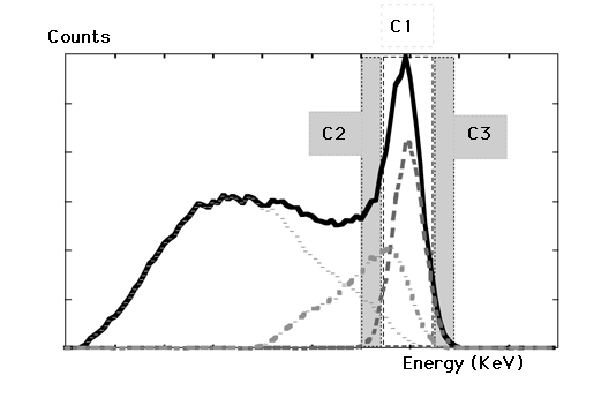
\includegraphics[width=0.5\textwidth]{figs/fig_TEW_scatter.pdf}
\caption{\label{fig:TEW_scatter} \emph{Triple energy window correction. The
amount of scattered photons accepted in window C1 is estimated as a fraction
of the counts in windows C2 and C3.}}
\end{figure}

\subsection{PET camera} \label{sec:petscatcor}
%----------------------
Just like the gamma camera, the PET camera uses a primary energy
window to reject photons with an energy that is clearly different from
511 keV. However, the energy resolution of current PET systems is
poorer than that of the gamma camera (15$\ldots$20\%). Unfortunately,
with poorer energy resolution, scatter correction based on an
additional energy window is less accurate. The reason is that the
center of the scatter window C2 has to be shifted farther away from
the primary energy peak, here 511 keV. Hence, the photons in that
window have lost more energy, implying that they have been scattered
over larger angles. Consequently, they are a poorer estimate of the
scatter inside the primary window, which has been scattered over
smaller angles.

For that reason, PET systems use a different approach to scatter
correction. As will be seen in chapter \ref{ch:trans}, PET scanners
are capable of measuring the attenuation coefficients of the patient
body. This can be used to calculate an estimate of the Compton scatter
contribution, if an estimate of the tracer distribution is available,
and if the characteristics of the PET system are known. Such
computations are done with Monte Carlo simulation. The simulator
software ``emits'' photons in a similar way as nature does: more
photons are emitted where more activity is present, and the photons
are emitted in random (pseudo-random in the software) directions. In a
similar way, photon-electron interactions are simulated, and each
photon is followed until it is detected or lost for detection
(e.g. because it flies in the wrong direction). This must be repeated
for a sufficient amount of photons, in order to generate a reasonable
estimate of the scatter contribution. Various clever tricks have been
invented to accelerate the computations, such that the whole procedure
can be done in a few minutes.

In practice, the method works as follows. First, a reconstruction of
the tracer uptake without scatter correction is computed. Based on
this tracer distribution and on the attenuation image of the patient,
the scatter contribution to the measured data is estimated with the
simulation software. This scatter contribution can then be subtracted
to produce a better reconstruction of the tracer distribution. This
procedure can be iterated to refine the scatter estimate.

\begin{figure}[tb]
\centering
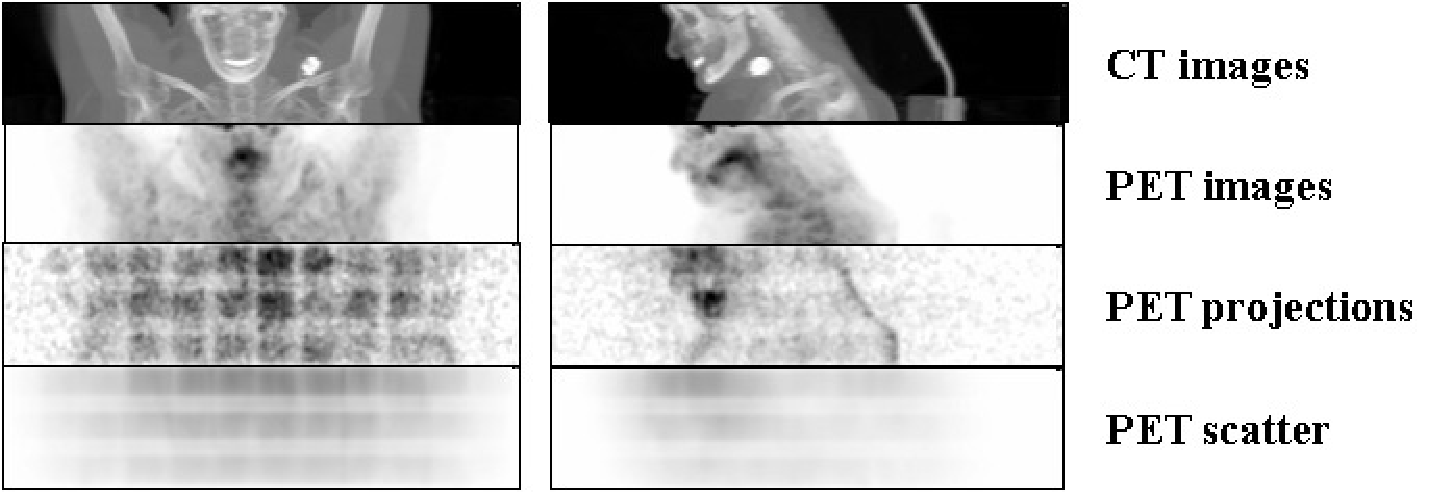
\includegraphics[width=0.9\textwidth]{figs/fig_pet_scatter.pdf}
\caption{\label{fig:petscatter} \emph{CT and PET images (obtained by
    maximum intensity projection), and the corresponding raw PET
    projection data with their estimated scatter contribution. Data
    were acquired with a Biograph 16 PET/CT system (Siemens). The
    regular pattern in the raw data is due to sensitivity differences
    between different detector pairs (see also fig \ref{fig:pet_norm}).}}
\end{figure}

Figure \ref{fig:petscatter} gives an example of the original raw PET
data from a 3D PET scan (slightly smoothed so you would see
something), together with the corresponding estimated scatter
contribution (using the same gray scales). Maximum intensity
projections of the CT and PET images are shown as well. The regular
pattern in the raw PET data is due to position dependent sensitivities
of the detector pairs (see also fig. \ref{fig:pet_norm}). The scatter
distribution is smooth, and its amplitude is significant.


\section{Other corrections} \label{sec:corrections}
%%%%%%%%%%%%%%%%%%%%%%%%%%%%%%%%%%
% Typische gamma camera
% Typische PET camera
% Linearity
% Energy
% Uniformity
% Dead time
%---
Currently, most gamma camera designs are based on a single crystal detector
as shown in figure \ref{fig:gammacamera}. To increase the sensitivity, a
single gamma camera may have two or three detector heads, enabling
simultaneous acquisition of two or three views along different angles
simultaneously. Because the detector head represents a significant portion of
the cost of the gamma camera, the price increases rapidly with the number of
detector heads.

Most PET systems have a multi-crystal design, they consist of multiple rings
(fig \ref{fig:jnpet}) of small detectors. The detectors are usually arranged
in modules (fig \ref{fig:multicrystal}) to reduce the number of PMT's.

The performance of the PMT's is not ideal for our purposes, and in addition
they show small individual differences in their characteristics. In current
gamma cameras and PET cameras the PMT-gain is computer controlled and
procedures are available for automated PMT-tuning. But even after tuning,
small differences in characteristics are still present.  As a result, some
corrections are required to ensure that the acquired information is reliable.

\begin{figure}[tb]
\centering
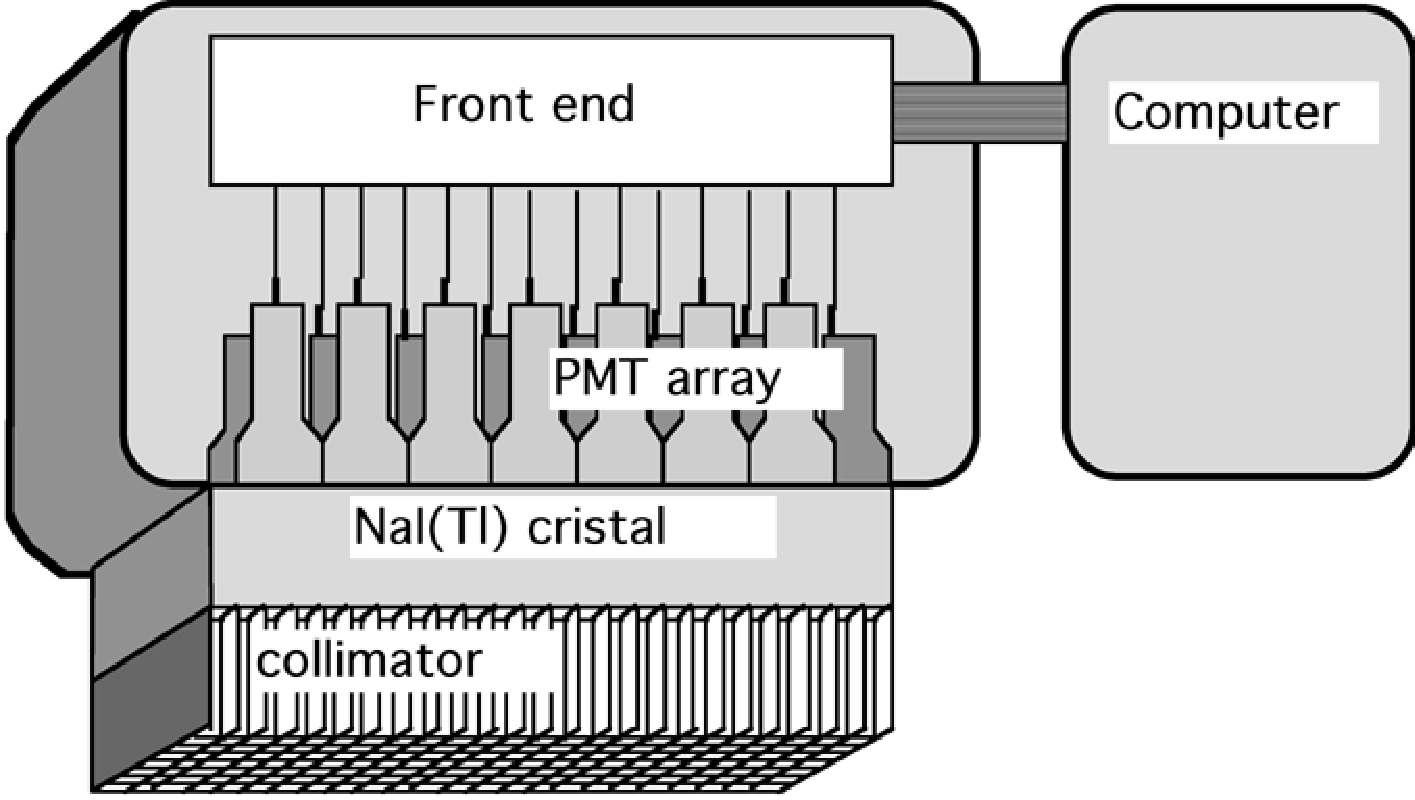
\includegraphics[width=0.5\textwidth]{figs/fig_jngamma.pdf}
\caption{\label{fig:gammacamera} \emph{Schematic representation of a gamma
camera with a single large scintillation crystal and parallel hole
collimator.}}
\end{figure}

\subsection{Linearity correction}
%=================================
\begin{figure}[tb]
\centering
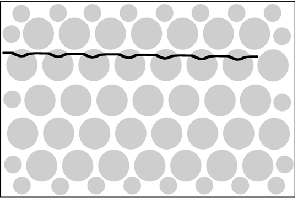
\includegraphics[width=0.5\textwidth]{figs/fig_linearity.pdf}
\caption{\label{fig:linearity} \emph{The PMTs (represented as circles) have a
non-linear response as a function of position. As a result, the image of a
straight radioactive line would be distorted as in this drawing.}}
\end{figure}

In section \ref{sec:single_crystal} we have seen that the position of
a scintillation in a large crystal is computed as the first moment in
$x$ and $y$ directions (the ``mass'' center of the PMT response). This
would be exact if the PMT response would vary linearly with
position. In reality, the response is not perfectly linear, and as a
result, the image is distorted. Figure \ref{fig:linearity} illustrates
how the image of a straight radioactive wire can be deformed by this
non-linear response. The response is systematic, so it can be
measured, and the errors $\Delta_x$ and $\Delta_y$ can be stored as a
function of $x$ and $y$ in a lookup table. Correction is then
straightforward:
\begin{align}
 x_{\text{corrected}} &= x + \Delta_x(x,y) \nonumber \\
 y_{\text{corrected}} &= y + \Delta_y(x,y)
\end{align}
After correction, the image of a straight line will be a straight line.

For a system using multi-crystal detectors, the linearity correction must be
applied within the modules, to make sure the correct individual detector is
identified. Because we know exactly where each module and each detector is
located, no further spatial corrections are required.

Because the system characteristics vary slowly in time, the linearity
correction table needs to be measured every now and then. This is typically
once a year or after a major intervention (e.g. after PMTs have been
replaced).

To measure the linearity, we must make an image of a {\em phantom}, a well
known object. One approach is to use a ``dot-phantom'': the collimator is
replaced with a lead sheet containing a matrix of small holes at regular
positions. Then we put some activity in front of the sheet (e.g. we can use a
point source at a large distance from the sheet), ensuring that all holes
receive approximately the same amount of photons. With this set up, an image
is acquired. Deviations between the image and the known dot pattern allow to
compute $\Delta_x(x,y)$ and $\Delta_y(x,y)$.

\subsection{Energy correction}
%=================================
Recall that the energy of the detected photon was computed as the sum of all
PMT responses (section \ref{sec:single_crystal}). Of course, the sum is
dominated by the few PMTs close to the point of scintillation, the other PMT's
receive very few or even no scintillation photons. Because the
PMT-characteristics show small individual differences, the computed energy is
position dependent. This results in small shifts of the computed energy
spectrum with position. The deviations are systematic (they vary only very
slowly in time), so they can be measured and stored, so that a position
dependent correction can be applied:
\begin{equation}
  E_{\mbox{corrected}}(x,y) = E(x,y) + \Delta_E(x,y)
\end{equation}

It is important that the energy window is nicely symmetrical around the
photopeak, small shifts of the window result in significant changes in the
number of accepted photons (figure \ref{fig:energy_corr}). Consequently, if no
energy correction is applied, the sensitivity for acceptable photons would be
position dependent.

\begin{figure}[tb]
\centering
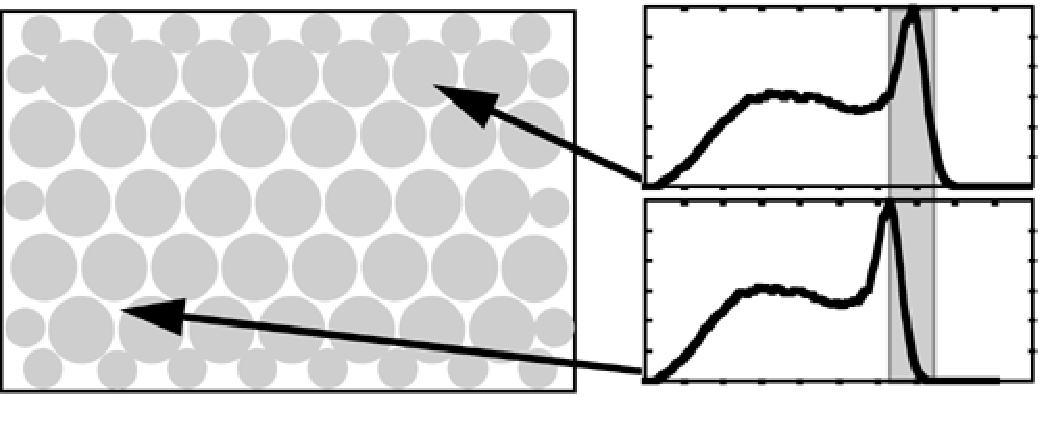
\includegraphics[width=0.5\textwidth]{figs/fig_energy_corr.pdf}
\caption{\label{fig:energy_corr} \emph{Because the characteristics of the
photomultipliers are not identical, the conversion of energy to voltage (and
therefore to a number in the computer) may be position dependent.}}
\end{figure}

The energy correction table needs to be rebuilt about every six months or
after a major intervention. The situation is similar for single crystal and
multicrystal systems.

%%%% TOT HIER NAGEZIEN.

\subsection{Uniformity correction}
%=================================
When linearity and energy correction have been applied, the image of a uniform
activity distribution should be a uniform image. In practice, there may still
be small differences, due to small variations of the characteristics with
position (e.g. crystal transparency, optical coupling between crystal and PMT
etc). Most likely, those are simply differences in sensitivity, so they do not
produce deformation errors, only multiplicative errors. Again, these
sensitivity changes can be measured and stored in order to correct them.

\subsubsection{Gamma camera}
%---------------------------
To measure the uniformity of the detector, we acquire an image of
a uniform activity. For the gamma camera, one approach is to put a
large homogeneous activity in front of the collimator. Another
possibility is to remove the collimator and put a point source at a
large distance in front of the collimator. Let us assume that the
point source is exactly in front of the center of the detector, at a
distance $H$ from the crystal. The number of photons arriving in
position $(x,y)$ per second and per solid angle is then
\begin{equation}
  \mbox{counts  per s and per solid angle} 
     = \frac{A}{4 \pi (H^2 + (x-x_0)^2 +(y-y_0)^2)}
\end{equation}
where $A$ is the strength of the source in Bq (Becquerel), and $(x_0, y_0)$ is
the center of the crystal. However, we don't need the number of
photons per solid angle, but the number of photons per detector
area. At position $(x,y)$, the photons arrive at an angle 
$\alpha = \arctan(\sqrt{(x-x_0)^2 +(y-y_0)^2}/ H)$. Thus, the solid
angle occupied by a small square of detector $dx\ dy$ equals $dx\ dy
\cos(\alpha)$. Because $\cos(\alpha) = H / \sqrt{H^2 + (x-x_0)^2
  +(y-y_0)^2}$, we obtain for the number of photons detected in $dx\
dy$:
\begin{equation}
  \mbox{counts detected in dx dy} 
     = \frac{A H}{4 \pi (H^2 + (x-x_0)^2 +(y-y_0)^2)^{3/2}}
     = \frac{A \cos^3\alpha}{H^2}
\end{equation}
%
Thus, if we know the size of the detector and the uniformity error we
will tolerate we can compute the required distance $H$.  You can
verify that with $H = 5 D$, where $D$ is the length of the crystal diagonal,
the maximum error equals about 1.5\%.

The number of photons detected in every pixel is Poisson distributed. Recall
from section \ref{sec:statistics} that the standard deviation of a Poisson
number is proportional to the square root of the expected value. So if we
accept an error (a standard deviation) of 0.5\%, we need to continue the
measurement until we have about 40000 counts per pixel. Computation of the
uniformity correction matrix is straightforward:
\begin{equation}
  \mbox{sensitivity\_corr}(x,y) = \frac{\mbox{mean}(I)}{I(x,y)}
\end{equation}
where $I$ is the acquired image.

Consequently, if a uniformity correction is applied to a planar image, one
Poisson variable is divided by another one. The relative noise variance in
the corrected image will be the sum of the relative noise variances on the
two Poisson variables (see appendix \ref{app:error} for estimating the error
on a function of noisy variables).

\subsubsection{PET camera} \label{sec:normalization1}
%-------------------------
In PET-vocabulary, uniformity correction is often called {\em detector
normalization}. The approach is similar as for the gamma camera, but
it is more difficult to measure the relative sensitivity of each
projection line than it is for a gamma camera.  One approach is to
slowly rotate a flat homogeneous phantom in the field of view, and
only use measurements along projection lines (nearly) perpendicular to
the phantom. It is time consuming, since most of the acquired data is
ignored, but it provides a direct sensitivity measurement for all
projection lines.

Alternatively, an indirect approach can be used. A sinogram is acquired for a
large phantom in the center of the field of view. All individual detectors
contribute to the measurement, and each detector is involved in multiple
projection lines intersecting the phantom. However, many other detector pairs
are not receiving photons at all. This measurement is sufficient to compute
individual detector sensitivities. Sensitivity of a projection line can then
be computed from the individual detector sensitivity and the known geometry.
The result is a sinogram representing projection line sensitivities. This
sinogram can be used to compute a correction for every sinogram pixel:
\begin{equation}
  \mbox{normalization}(i) = 
    \frac{\mbox{mean(sensitivity)}}{\mbox{sensitivity}(i)}. \label{eq:petnorm}
\end{equation}
A typical sensitivity sinogram is shown in figure
\ref{fig:pet_norm}. The sinogram is dominated by a regular pattern of
zero sensitivity projection lines, which are due to small gaps between
the detector blocks. In the projections one can see that there is a
significant axial variation in the sensitivities. After normalization,
the data from a uniform cylinder are indeed fairly uniform, except for
these zero sensitivities. In iterative reconstruction, the data in
these gaps are simply not used. For filtered backprojection, these
data must first be filled with some interpolation algorithm.
%
\begin{figure}[tb]
\centering
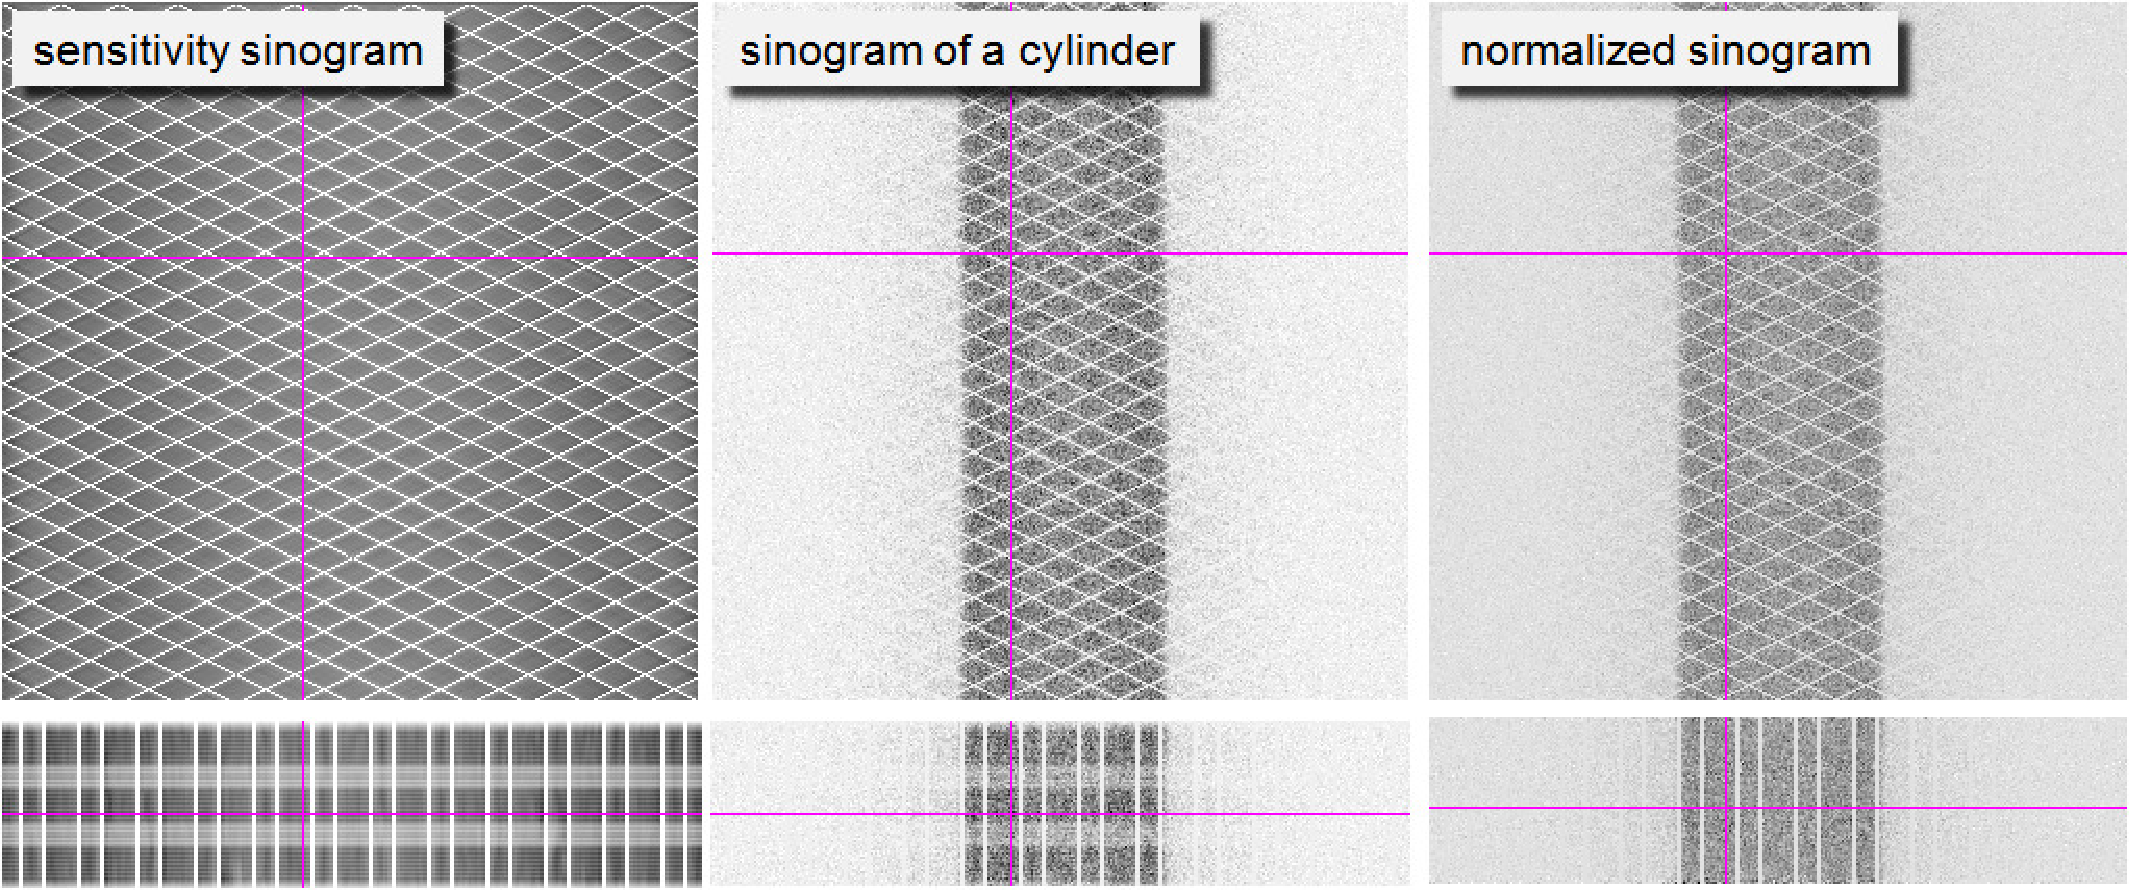
\includegraphics[width=0.9\textwidth]{figs/fig_PETsens.pdf}
\caption{\label{fig:pet_norm} \emph{Left: PET sensitivity
    sinogram. Center: the sinogram of a cylinder filled with a uniform
    activity. Right: the same sinogram after normalization. The first
    row are sinograms, the second row projections, the cross-hairs
    indicate the relative position of both. Because there are small
    gaps between detector blocks, there is a regular pattern of zero
    sensitivity projection lines, which are of course not corrected by the
    normalization.}}
\end{figure}


\subsection{Dead time correction} \label{sec:deadtime}
%=================================
``Dead time'' means that the system has a limited data processing capacity. If
the data input is too high, a fraction of the data will be ignored because of
lack of time. As a result, the measured count rate is lower than the true
count rate, and the error increases with increasing true count rate. Figure
\ref{fig:dead_time} shows the measured count rate as a function of the true
count rate for a dead time of 700 ns. The gamma camera and the PET camera both
have a finite dead time, consisting of several components. To describe the
dead time, we will assume that all contributions can be grouped in two
components, a front-end component and a data-processing component.

\begin{figure}[tb]
\centering
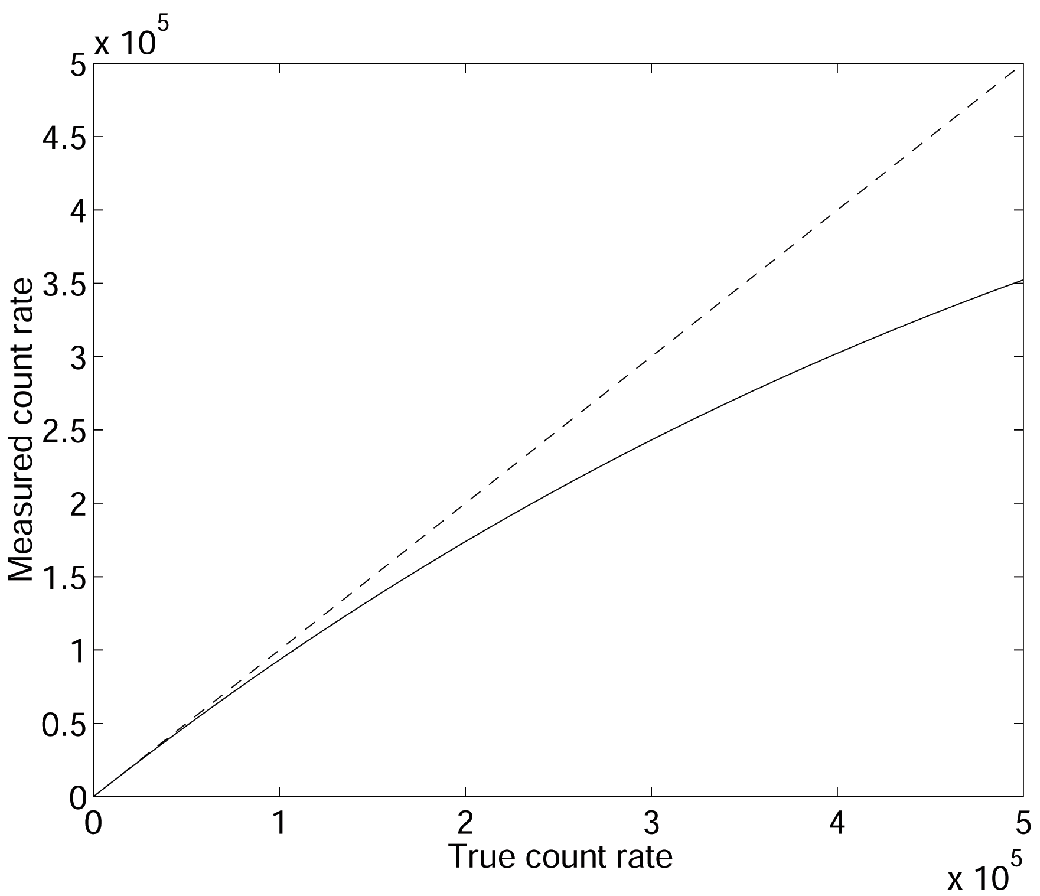
\includegraphics[width=0.5\textwidth]{figs/fig_dead_time.pdf}
\caption{\label{fig:dead_time} \emph{Due to dead time, the measured count rate
is lower than the true count rate for high count rates. The figure is for a
dead time of 700 ns, the axes are in counts per second. Measured count rate is
20\% low near 300000 counts per second.}}
\end{figure}

\subsubsection{Front-end dead time}
%------------------------------------
Recall (section \ref{sec:single_crystal}) that the scintillation has
a finite duration. E.g., the decay time of NaI(Tl) is 230 ns. The PMT
response time adds a few ns. To have an accurate estimate of the
energy, we need to integrate over a sufficient fraction of the
PMT-outputs, such that most of the scintillation photons get the
chance to contribute. Let us assume that the effective scintillation
time is $\tau_1 / 2$, and that we integrate over that time to compute
position and energy. Then the result is only correct if no new
scintillation starts during that period, and no old one is ending
during that period (so the previous scintillation must be older than
$\tau_1/2$).  Otherwise, part of this other scintillation will
contribute as well, the energy will be overestimated and the photon is
rejected. Consequently, a photon is only detected if in a time
$\tau_1$ exactly one photon arrives.  If we have a true count rate of
$R_0$, then we expect $R_0 \tau_1$ photons in the interval
$\tau_1$. Recall that the number of photons is Poisson distributed, so
the probability of having 1 photon when $R_0 \tau_1$ are expected is
$\exp(- R_0 \tau_1) R_0 \tau_1$. This is the count per time $\tau_1$,
so the count rate of accepted events will be
\begin{equation}
  R_1 = R_0 e^{-R_0 \tau_1}. \label{eq:deadtime_front}
\end{equation}
Notice that if $R_0$ is extremely large, $R_1$ goes to zero: the system is
said to be {\em paralyzable}. Indeed, if the count rate is extremely high,
every scintillation will be disturbed by the next one, and the camera will
accept no events at all.

\subsubsection{Data-processing dead time}
%------------------------------------
When the event is accepted, the linearity correction must be applied and it
must be stored somehow: the electronics either stores it in a list, and
increments the pointer to the next available address, or it increments the
appropriate location in the image. This takes time, let us say $\tau_2$. If
during that time another event occurs, it is simply ignored. Consequently, a
fraction of the incoming events will be missed, because the electronics is not
permanently available.

Assume that the electronics needs to store data at a rate of $R_2$ (unit
$s^{-1}$). Each of these requires $\tau_2$ s, so in every second, $R_2 \tau_2$
are already occupied for processing data. The efficiency of the system is
therefore $1 - \tau_2 R_2$, which gives us the relation between incoming count
rate $R_1$ and processed count rate $R_2$:
\begin{equation}
  R_2 = (1 - R_2 \tau_2) R_1
\end{equation}
Rearranging this to obtain $R_2$ as a function of $R_1$ results in
\begin{equation}
  R_2 = \frac{R_1}{1 + R_1 \tau_2}. \label{eq:deadtime_proc}
\end{equation}
This function is monotonically increasing with upper limit $1 /
\tau_2$ (as you would expect: this is the number of intervals of
length $\tau_2$ in one second).  Consequently, the electronics is
non-paralyzable. You cannot paralyze it, but you can saturate it: if
you put in too much data, it simply performs at maximum speed ignoring
all the rest.

\subsubsection{Effective dead time}
%------------------------------------
Combining (\ref{eq:deadtime_front}) and (\ref{eq:deadtime_proc}) tells us the
acceptance rate for an incident photon rate of $R_0$:
\begin{equation}
  R_2 = \frac{R_0 e^{-R_0 \tau_1}}{ 1 + R_0 e^{-R_0 \tau_1} \tau_2}.
\end{equation}
If the count rates are small compared to the dead times (such that $R_x
\tau_y$ is small), we can introduce an approximation to make the
expression simpler. The approximation is based on the following relations,
which are acceptable if $x$ is small:
\begin{align}
  e^{-x} &\simeq e^{-0} + x \left. \frac{d e^{-x}}{dx} \right|_{x=0}= 1-x\\
         &= \frac{1+x}{1+x} - x = \frac{1+x-x-x^2}{1+x} 
        \simeq \frac{1}{1 + x}.
\end{align}
Applying this to (\ref{eq:deadtime_front}) and (\ref{eq:deadtime_proc}) yields:
\begin{align}
  R_1 &\simeq R_0 (1 - R_0 \tau_1)\\
  R_2 &\simeq R_1 (1 - R_1 \tau_2)
\end{align}
Combining both equation and deleting higher order terms results in
\begin{align}
  R_2 &\simeq R_0 \left(1 - R_0 (\tau_1 + \tau_2) \right) \label{eq:dead1}\\
      &\simeq R_0 e^{- R_0 (\tau_1 + \tau_2)} \label{eq:dead2}
\end{align}
So if the count rate is relatively low, there is little difference between
paralyzable and non-paralyzable dead time, and we can obtain a global dead
time for the whole machine by simply adding the contributing dead times.  Most
clinical gamma cameras and all PET systems provide dead time correction based
on some dead time model. However, for very high count rates the models are no
longer valid and the correction will not be accurate.

\subsection{Random coincidence correction} \label{sec:randoms}
%=========================================
The random coincidence was defined in section \ref{sec:petcollim}: two
non-related events may be detected simultaneously and be interpreted as a
coincidence. There is no way to discriminate between true and random
coincidences. However, there is a ``simple'' way to measure a reliable
estimate of the number of randoms along every projection line. This is done
via the delayed window technique.

The number of randoms (equation (\ref{eq:pet_randoms})) was obtained by
squaring the probability to measure a single event during a time window
$\tau$. In the delayed window technique, an additional time window is used,
which is identical in length to the normal one but delayed over a short time
interval. The data for the second window are monitored with the same
coincidence electronics and algorithms as used for the regular coincidence
detection, ignoring the delay between the windows. If a coincidence is
obtained between an event in the normal and an event in the delayed window,
then we know it has to be a random coincidence: because of the delay the
events cannot be due to the same annihilation. Consequently, with regular
windowing we obtain {\em trues + randoms1}, and with the delayed method we
obtain a value {\em randoms2}. The values {\em randoms1} and {\em randoms2}
are not identical because of Poisson noise, but at least their expectations
are identical. Subtraction will eliminate the bias, but will increase the
variance on the estimated number of trues. See appendix \ref{app:error} for
some comments on error propagation.